%%
%% Copyright 2007, 2008, 2009 Elsevier Ltd
%%
%% This file is part of the 'Elsarticle Bundle'.
%% ---------------------------------------------
%%
%% It may be distributed under the conditions of the LaTeX Project Public
%% License, either version 1.2 of this license or (at your option) any
%% later version.  The latest version of this license is in
%%    http://www.latex-project.org/lppl.txt
%% and version 1.2 or later is part of all distributions of LaTeX
%% version 1999/12/01 or later.
%%
%% The list of all files belonging to the 'Elsarticle Bundle' is
%% given in the file `manifest.txt'.
%%

%% Template article for Elsevier's document class `elsarticle'
%% with numbered style bibliographic references
%% SP 2008/03/01
%%
%%
%%
%% $Id: elsarticle-template-num.tex 4 2009-10-24 08:22:58Z rishi $
%%
%%
\documentclass[preprint,12pt]{elsarticle}

%% Use the option review to obtain double line spacing
%% \documentclass[preprint,review,12pt]{elsarticle}

%% Use the options 1p,twocolumn; 3p; 3p,twocolumn; 5p; or 5p,twocolumn
%% for a journal layout:
%% \documentclass[final,1p,times]{elsarticle}
%% \documentclass[final,1p,times,twocolumn]{elsarticle}
%% \documentclass[final,3p,times]{elsarticle}
%% \documentclass[final,3p,times,twocolumn]{elsarticle}
%% \documentclass[final,5p,times]{elsarticle}
%% \documentclass[final,5p,times,twocolumn]{elsarticle}

%% if you use PostScript figures in your article
%% use the graphics package for simple commands
%% \usepackage{graphics}
%% or use the graphicx package for more complicated commands
\usepackage{amsmath,amssymb,amsfonts,stmaryrd,amsthm}
\usepackage{algorithm}
\usepackage{algorithmic}
\usepackage{graphicx}
\usepackage{pstricks}
\usepackage{eepic}
\usepackage{float}

%% or use the epsfig package if you prefer to use the old commands
%% \usepackage{epsfig}

%% The amssymb package provides various useful mathematical symbols
%\usepackage{amssymb}
%% The amsthm package provides extended theorem environments
%% \usepackage{amsthm}

%% The lineno packages adds line numbers. Start line numbering with
%% \begin{linenumbers}, end it with \end{linenumbers}. Or switch it on
%% for the whole article with \linenumbers after \end{frontmatter}.
%% \usepackage{lineno}

%% natbib.sty is loaded by default. However, natbib options can be
%% provided with \biboptions{...} command. Following options are
%% valid:

%%   round  -  round parentheses are used (default)
%%   square -  square brackets are used   [option]
%%   curly  -  curly braces are used      {option}
%%   angle  -  angle brackets are used    <option>
%%   semicolon  -  multiple citations separated by semi-colon
%%   colon  - same as semicolon, an earlier confusion
%%   comma  -  separated by comma
%%   numbers-  selects numerical citations
%%   super  -  numerical citations as superscripts
%%   sort   -  sorts multiple citations according to order in ref. list
%%   sort&compress   -  like sort, but also compresses numerical citations
%%   compress - compresses without sorting
%%
%% \biboptions{comma,round}

% \biboptions{}


\journal{SINUM}

\newtheorem{theorem}{Theorem}[section]
\newtheorem{lemma}[theorem]{Lemma}
\newtheorem{corollary}[theorem]{Corollary}
\newtheorem{definition}[theorem]{Definition}
\newtheorem{assumption}[theorem]{Assumption}

\newcommand{\cS}{\mathcal{S}}
\newcommand{\tU}{\tilde{U}}
\newcommand{\ta}{\tilde{a}}
\newcommand{\tk}{\tilde{k}}
\newcommand{\bfb}{\mathbf{b}}
\newcommand{\tB}{\tilde{\mathcal{B}}}
\newcommand{\cV}{\mathcal{V}}
\newcommand{\cT}{\mathcal{T}}
\newcommand{\calB}{\mathcal{B}}
 \newcommand{\cB}{{B}}
\newcommand{\cL}{\mathcal{L}}
\newcommand{\cK}{\mathcal{K}}
\newcommand{\cE}{\mathcal{E}}
\newcommand{\cI}{\mathcal{I}}
\newcommand{\cA}{{A}}
\newcommand{\calA}{\mathcal{A}}
\newcommand{\cO}{\mathcal{O}}
\newcommand{\osc}{\mathrm{osc}}
\newcommand{\R}{\mathbb{R}}
\newcommand{\N}{\mathbb{N}}
\newcommand{\bk}{\mathbf{k}}
\newcommand{\br}{\mathbf{r}}
\newcommand{\tcb}{\textcolor{blue}}


\begin{document}

\begin{frontmatter}

%% Title, authors and addresses

%% use the tnoteref command within \title for footnotes;
%% use the tnotetext command for the associated footnote;
%% use the fnref command within \author or \address for footnotes;
%% use the fntext command for the associated footnote;
%% use the corref command within \author for corresponding author footnotes;
%% use the cortext command for the associated footnote;
%% use the ead command for the email address,
%% and the form \ead[url] for the home page:
%%
%% \title{Title\tnoteref{label1}}
%% \tnotetext[label1]{}
%% \author{Pavel Solin\corref{cor1}\fnref{label2}}
%% \ead{solin@unr.edu}
%% \ead[url]{http://hpfem.org/\tilde pavel}
%%\fntext[label2]{}
%% \cortext[cor1]{}
%% \address{\fnref{label3}}
%% \fntext[label3]{}

%\title{Picard and Newton-Based Adaptive Finite Element Methods for Eigenvalue Problems}
\title{Adaptive $hp$-FEM for Eigenvalue Problems\\ Free of Repeated 
       Eigensolver Calls}

%% use optional labels to link authors explicitly to addresses:
\author[label1,label2]{Pavel Solin}
\ead{solin@unr.edu}
\author[label3]{Stefano Giani}
\ead{stefano.giani@nottingham.ac.uk}
\address[label1]{Department of Mathematics and Statistics, University of Nevada, Reno, USA}
\address[label2]{Institute of Thermomechanics, Academy of Sciences of the Czech Republic, Prague}
\address[label3]{School of Mathematical Sciences, University of Nottingham, United Kingdom}


%\address{Department of Mathematics and Statistics, University of Nevada, Reno, USA}

\begin{abstract}

Conventional adaptive finite element methods (FEM) for eigenvalue problems call 
an eigensolver in each adaptivity step. This is not optimal in all situations, 
for example if one is only interested in resolving accurately one specific 
vibration mode. We propose a novel adaptive algorithm that only calls the 
eigensolver once at the beginning of the computation, and then employs an 
iterative method to converge to any selected eigenvalue-eigenvector pair. 
Picard and Newton variants of such an iterative method are presented. 
In the case that the eigenvalue-eigenvector pair of interest is part of a multiple eigenvalue,
we propose a method to track the same eigenpair on all the successive adapted meshes.
The 
underlying partial differential equation (PDE) is discretized with higher-order 
finite elements ($hp$-FEM) but the algorithm also works for standard 
low-order FEM. The method is described and accompanied with theoretical 
analysis and numerical examples and comparisons. Instructions on how to 
reproduce the results are provided. 
\end{abstract}

\begin{keyword}
Partial differential equation \sep Eigenvalue problem \sep Adaptive higher-order finite element
method \sep $hp$-FEM \sep Reproducible research
%% keywords here, in the form: keyword \sep keyword
%% MSC codes here, in the form: \MSC code \sep code
%% or \MSC[2008] code \sep code (2000 is the default)
\end{keyword}

\end{frontmatter}

%%
%% Start line numbering here if you want
%%
% \linenumbers

%% main text
%\section{Introduction}

%\begin{itemize}
%\item Give examples of applications where accurate approximation of  
%      a single eigenfunction is useful.
%\item Mention applications where simultaneous approximation of
%      several eigenfunctions is needed (I know about DFT. Is there something else?). 
%      \textcolor{red}{I could suggest Photonic Crystal problems, it is necessary to compute several eigenvalues in order to identify gaps in the spectrum of the problem}
%\item Give references to prior work on adaptive algorithms for 
%      PDE eigenproblems, limitations, ... We have to show that we are aware of 
%      latest developments.
%\end{itemize}

\section{Introduction}\label{sec:intro}

The eigenvalue problem are of considerable theoretical interest and wide-ranging applications.
They arise naturally in many physical processes 
and they have a lot of applications in physics and engineering. For example, a lot of problems in acoustics can be expressed as an eigenvalue problem or eigenvalue problems are solved inside many methods like in automated multilevel substructuring for noise prediction \cite{lalor_prediction_2007}.
Nano-optics is another field where eigenvalue problems can be found very often, the analysis of photonic crystals \cite{pcf_apost,JoMeWi:95} and plasmonic guides \cite{berini_plasmon-polariton_2000} are based on them. 
Another example where eigenvalue problems are used is the study of stability of fluid dynamics systems \cite{cliffe_adaptive_2010}
%Example of applications 
%are in structural engineering, weather forecasting and in quantum physics. {\red Pavel, I'm still looking for references} 
The most common approach to solve an eigenproblem in practice is use an eigensolver, and for problem large enough an iterative one, like ARPACK \cite{arpack}, is used.
A characteristic common to all eigensolver is that, even if the user is interested in one particular eigenpair, a bunch of unwanted eigenvalue and possibly eigenvectors is computed in order for the eigensolver to work. These unwanted eigenpair are the byproduct of techniques such as deflation or 
orthogonalization used to filter out unwanted solutions.
Also the great majority of eigensolvers are not specifically designed to work with adaptive finite elements or finite differences methods. Therefore we propose a different approach based on simple and widely used iterative methods for non-linear problems. We are going to adapt the Picard's and the Newton's method to solve eigenvalue problems and we minimize the number of computed unwanted eigenpair exploiting the orthogonality between eigenvectors. Also, a method to compute the approximation of the same eigenpair on a sequence of adapted meshes is presented. This method is particularly useful with multiple eigenvalues when only a particular eigenfunction in the eigenspace is wanted. 

%The outline of the paper is as follows. In Section~\ref{sec:motiv} we describe the motivation for this paper and in Section~\ref{sec:pre} we introduce the model problem considered in this work. Then in Sections~\ref{sec:motiv} and \ref{sec:motiv} we introduce our first iterative method base on the Picard's method.
%Similarly, in Section~\ref{sec:newton} we introduce our first iterative method base on the Newton's method. Then in Sections~\ref{sec:rec} and \ref{sec:rec2} we describe a method to follow the target eigenpair on a sequence of adaptively refined meshes. Moreover, in Section~\ref{sec:imp_ortho} we present improved versions of our iterative methods. We conclude the theoretical part of the paper with Section~\ref{sse:pcf_priori}, where the a priori convergence results for the methods are presented.
%Finally, in Section~\ref{sec:num} numerical results are discussed and in Section~\ref{sec:reproducibility} the settings of the numerical experiments are described.


%{\red STEFANO, could you please write an introduction that acknowledges 
%previous work on adaptive FEM for eigenproblems? In particular, we should cite people that we 
%suggest as referees. The conclusion should be that it is customary to  
%call the eigensolver in each adaptivity step.}

\subsection{Outline of the Paper}

Section \ref{sec:motiv} illustrates difficulties associated with 
adaptive methods that need to call an eigensolver in each adaptivity 
step. Section \ref{sec:preli} introduces some notations and 
preliminaries. Section \ref{sec:picard} presents a simple
Picard's method and shows that it does not work as expected.
The problem is fixed in Section \ref{sec:picard++} by adding 
orthogonalization. Section \ref{sec:newton} presents 
a Newton's method with orthogonalization. 
Section \ref{sec:adapt} presents an outline of the adaptivity algorithm,
which is needed in the following section.
Section \ref{sec:reco}
discusses a reconstruction technology for spectra perturbed 
by discretization. This is used to devise an algorithm for 
computing reference solutions for $hp$-adaptivity in 
Section \ref{sec:recoref}. 
Moreover, in Section~\ref{sec:imp_ortho} we present improved versions of our iterative methods.A priori convergence results 
are presented in Section \ref{sec:aprio}. Numerical results 
are presented in Section \ref{sec:numer}. Reproducibility of 
results is discussed in Section \ref{sec:reproducibility}.
Conclusion and outlook are presented in Section \ref{sec:conclusion}.


\section{Motivation}\label{sec:motiv}

We will illustrate a typical outcome of repeated eigensolver calls
on a simple eigenproblem of the form 
\begin{equation} \label{one}
-\Delta u = \lambda u, \ \ \ u = 0 \ \mbox{on} \ \partial \Omega
\end{equation}
that is solved in a square domain $\Omega = (0, \pi)^2$.
In this case the eigenvalues $0 < \lambda_1 \le \lambda_2 \le \ldots$ 
are known exactly, and it is of particular interest that $\lambda_2 = \lambda_3 = 5$ 
and $\lambda_5 = \lambda_6 = 10$ are repeated. 

Equation (\ref{one}) is discretized via the finite element method
on a $4\times 4$ mesh consisting of quadratic elements shown in Fig. \ref{fig:mesh1}.\\

\begin{figure}[!ht]
\begin{center}
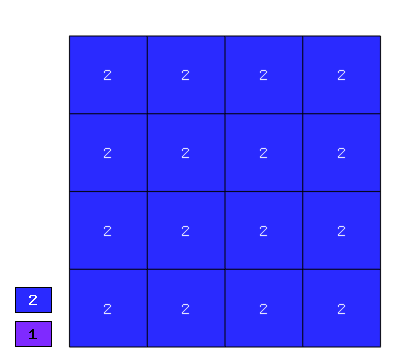
\includegraphics[width=0.36\textwidth]{img/mesh_1.png}
\end{center}
\vspace{-5mm}
\caption{Initial mesh for automatic adaptivity.}
\label{fig:mesh1}
\end{figure}

Here, the numbers inside of finite elements mean their polynomial degrees.
Approximate eigenfunctions for $\lambda_2, \lambda_3$ and $\lambda_5, \lambda_6$
are shown in the first and second row of Fig. \ref{fig:eigen1}, respectively.
%The reader can see that the eigenfunctions exhibit anisotropies that make it 
%impossible for a single finite element mesh to be optimal for all 
%of them simultaneously.

\clearpage

\begin{figure}[!ht]
\begin{center}
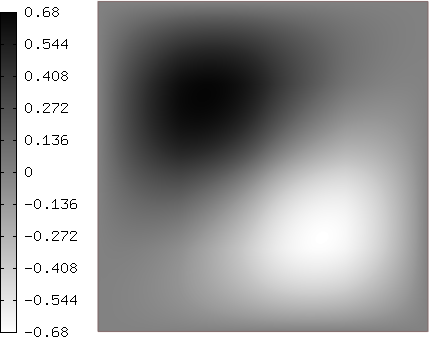
\includegraphics[width=0.4\textwidth]{img/eigen_1.png}\ \ \ 
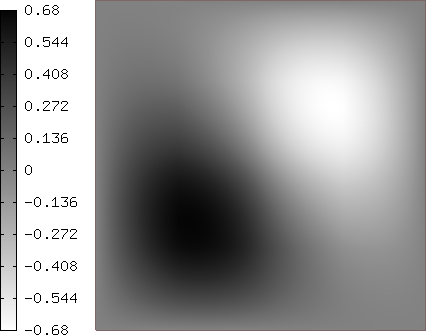
\includegraphics[width=0.4\textwidth]{img/eigen_2.png}\\[4mm]
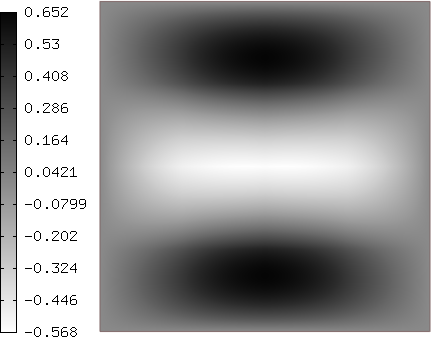
\includegraphics[width=0.4\textwidth]{img/eigen_3.png}\ \ \ 
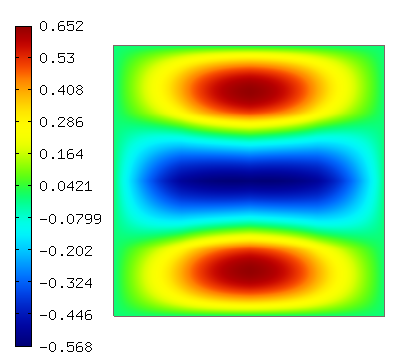
\includegraphics[width=0.4\textwidth]{img/eigen_4.png}\\
\end{center}
\vspace{-5mm}
\caption{Approximate eigenfunctions for $\lambda_2, \lambda_3$ and 
$\lambda_5, \lambda_6$ on initial mesh.}
\label{fig:eigen1}
\end{figure}

Assume that based on some a-posteriori error estimate, the mesh undergoes 
$p$-refinement of the four interior elements, as shown in Fig. \ref{fig:mesh2}.

\begin{figure}[!ht]
\begin{center}
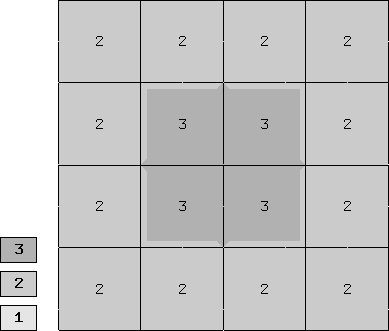
\includegraphics[width=0.36\textwidth]{img/mesh_2.png}
\end{center}
\vspace{-5mm}
\caption{Mesh after the first adaptivity step.}
\label{fig:mesh2}
\end{figure}

After refining the mesh, the eigensolver is called again. 
The resulting approximate eigenfunctions for $\lambda_2, \lambda_3$ and $\lambda_5, \lambda_6$
are shown in the first and second row of Fig. \ref{fig:eigen2}, respectively.

\clearpage
\begin{figure}[!ht]
\begin{center}
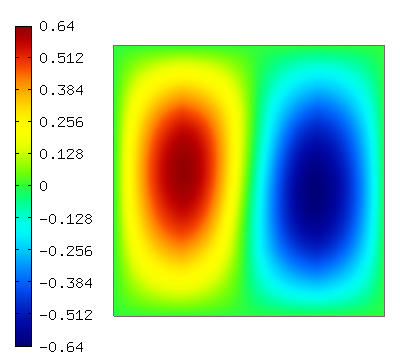
\includegraphics[width=0.4\textwidth]{img/eigen_5.png}\ \ \ 
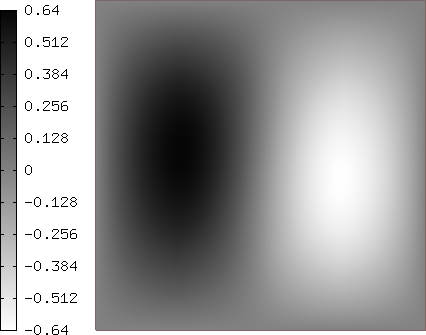
\includegraphics[width=0.4\textwidth]{img/eigen_6.png}\\[4mm]
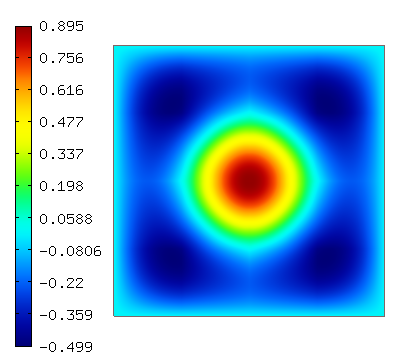
\includegraphics[width=0.4\textwidth]{img/eigen_7.png}\ \ \ 
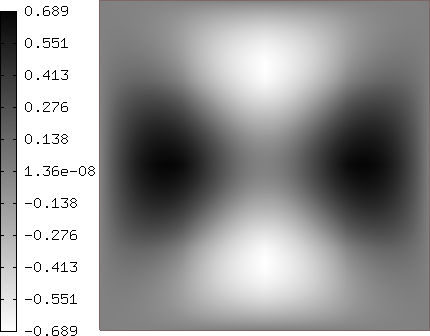
\includegraphics[width=0.4\textwidth]{img/eigen_8.png}\\
\end{center}
\vspace{-5mm}
\caption{Approximate eigenfunctions for $\lambda_2, \lambda_3$ and 
$\lambda_5, \lambda_6$ after the first adaptivity step.}
\label{fig:eigen2}
\end{figure}

The reader can observe that the approximations changed dramatically after the 
mesh was refined. This is known behavior that is due to the multiplicity of the 
corresponding eigenvalues. To our best knowledge, contemporary generalized 
eigensolvers do not offer any way to avoid this problem. 
{\red STEFANO, we have to be a bit careful here. Are there any works dealing 
with repeated eigenvalues? If so, we have to cite them here.} {\red Pavel, there are many works where eigenvalues are considered, sometimes also repeated eigenvalues are considered. I have a couple of papers containing numerics for repeated eigenvalues. 
But I wasn't able to find anything specific on multiple eigenvalues. 
Normally you just apply to repeated eigenvalues the same method that you use for simple ones.
Have you found anything?}
Instructions on how to reproduce 
these results are provided in Section \ref{sec:reproducibility}.

%%%%%%%%%%%%%%%%%%%%%%%%%%%%%%%%%%%%%%%%%%%%%%%%%%%%%%%%%%%%%%%%%%%%%%%%%%%%%%%%%%%%%%%%%%%%%%%%%%%%%%%%%

\section{Preliminaries}\label{sec:preli}

Throughout, $L^2(\Omega)$
denotes the usual space of square-integrable real valued functions
equipped with the standard norm
\begin{equation}\label{eq:l2}
\|f\|_{0}\ := \ \left(\int_\Omega  |f|^2\right)^{\frac{1}{2}} .
\end{equation}
The symbol $H^1(\Omega)$ denotes the usual space of functions in $L^2(\Omega)$
with square-integrable weak first partial derivatives. The $H^1$-norm is 
denoted by $\|f\|_1$.

The variational formulation of problem \eqref{one} is:
\emph{Find eigenpairs of the form $(\lambda_j,u_j)\in
\mathbb{R}\times H^1_0(\Omega)$
such that}
\begin{equation}
\label{eq:var_prob}
\left.
\begin{array}{lcl}
a(u_j,v)&=& \lambda_j\ b(u_j,v),
\quad \text{for all } \quad v  \in H^1_0(\Omega)\\
 \Vert u_j \Vert_{0} &=& 1
\end{array}\quad
\right\}
\end{equation}
where
\begin{equation}\label{eq:a}
a(u,v):=\int_\Omega \nabla u(x)\cdot \nabla v(x),
\end{equation}
and
\begin{equation}\label{eq:b}
b(u,v):=\int_\Omega u(x) v(x).
\end{equation}

Now, to discretize (\ref{eq:var_prob}), let $\cT_n, n =
1,2,\ldots $ denote a family of meshes on $\Omega$.
The meshes can be irregular with multiple levels of hanging nodes, 
and they can combine possibly curvilinear triangular and quadrilateral 
elements. These meshes may be obtained using automatic adaptivity. 

By $h_{n,\tau}$ we denote the diameter of element $\tau$,  
we define
$
h_n:=\max_{\tau\in \mathcal{T}_n}\{h_{n,\tau}\}.
$
Similarly with  $p_{n,\tau}$ we denote  the order of polynomials of element $\tau$,  
we define
$
p_n:=\min_{\tau\in \mathcal{T}_n}\{p_{n,\tau}\}.
$
On any mesh $\mathcal{T}_n$ we denote by $V_n \subset H^1_0(\Omega)$ the finite
dimensional space of continuous functions $v$ such that on any element $\tau$ we 
have that $v|_\tau\in \mathcal{P}_{p_{n,\tau}}(K)$. Here either $\mathcal{P}_{p_{n,\tau}}(K)$ 
is the space of polynomials of total degree at most $p_{n,\tau}$ if $\tau$ is a triangular 
element, or $\mathcal{P}_{p_{n,\tau}}(K)$ is the space of polynomials of degree at most 
$p_{n,\tau}$ in each variable if $\tau$ is a quadrilateral element.


%\textcolor{red}{I have to define better the meshes and the space and add references.}

The discrete version of \eqref{eq:var_prob} reads:
\emph{Find eigenpairs of the form $(\lambda_{j,n},u_{j,n})\in
\mathbb{R}\times V_n$
such that}
\begin{equation}
\label{eq:disc_prob}
\left.
\begin{array}{lcl}
a(u_{jn},v_{n})&=& \lambda_{j,n}\ b(u_{j,n},v_{n}),
\quad \text{for all } \quad v_{n}  \in V_n\\
 \Vert u_{j,n} \Vert_{0} &=& 1
\end{array}\quad
\right\}
\end{equation}

%%%%%%%%%%%%%%%%%%%%%%%%%%%%%%%%%%%%%%%%%%%%%%%%%%%%%%%%%%%%%%%%%%%%%%%%%%%%%%%%%%%%%%%%%%%%%%%%%%%%%%%%%

\section{Picard's Method}\label{sec:picard}

Problem \eqref{eq:disc_prob} can be reformulated in matrix format as:
\emph{seek eigenpairs of the form $(\lambda,\mathbf{u})\in
\mathbb{R}\times \mathbb{R}^N$, where $N$ is the dimension of $V_n$,
such that}
\begin{equation}
\label{eq:disc_prob_mat}
\left.
\begin{array}{lcl}
\mathbf{A} \mathbf{u}&=& \lambda\mathbf{B}\mathbf{u}\ ,
\\
\mathbf{u}^t\mathbf{B} \mathbf{u} &=& 1
\end{array}\quad
\right\}
\end{equation}
where the entries of the matrices $\mathbf{A}$ and $\mathbf{B}$ are 
$$
\mathbf{A}_{k,p}:=a(\phi_k,\phi_p)\ ,\quad\mathbf{B}_{k,p}:=b(\phi_k,\phi_p)\ ,
$$
where $\phi_i$ are the basis functions spanning $V_n$.

The Picard's method, see Algorithm~\ref{alg:picard}, takes as arguments the matrices $\mathbf{A}$ and $\mathbf{B}$, an initial guess $\tilde u$ for the eigenfunction, a relative tolerance $\mathrm{Tol}$ and an absolute tolerance $\mathrm{AbsTol}$. {\red Pavel, the introduction of $\mathrm{AbsTol}$ should make both iterative algorithm to converge and stop correctly.} The algorithm returns an approximated eigenpair $(\lambda_{n},u_{n})$.
Because we use this iterative method on a sequence of adaptively refined meshes, we normally set as initial guess
the projection in the refined mesh of the eigenfunction of interest $u_{j,n-1}$.

\begin{algorithm}[H] \caption{Picard's method} \label{alg:picard} 
\begin{algorithmic}

\STATE{$(\lambda_{j,n},u_{j,n}):=\mathrm{Picard}
    (\mathbf{A}, \mathbf{B},\tilde u,\mathrm{Tol},\mathrm{AbsTol})$}

\STATE{$\mathbf{u}^1:=\tilde u$}
\STATE{$\displaystyle\lambda^{1}:=\frac{u_{j,n}^t\mathbf{A}u_{j,n}}{u_{j,n}^t\mathbf{B}u_{j,n}}$}
\STATE{$m=1$}
\REPEAT

\STATE{$\mathbf{u}^{m+1}:=\mathbf{A}^{-1}\lambda^m\mathbf{B}\mathbf{u}^{m}$}
\STATE{$\displaystyle\lambda^{m+1}:=\frac{(\mathbf{u}^{m+1})^t\mathbf{A}\mathbf{u}^{m+1}}{(\mathbf{u}^{m+1})^t\mathbf{B}\mathbf{u}^{m+1}}$}
\STATE{$m:=m+1$}
\UNTIL{ $\frac{\|\mathbf{u}^{m+1}-\mathbf{u}^{m}\|_1}{\|\mathbf{u}^{m}\|_1}>\mathrm{Tol}$ \bf{and}
$|\lambda^{m+1}-\lambda^m|>\mathrm{AbsTol}$}
\STATE{$u_{n}:=\mathbf{u}^{m}$}
\STATE{$\lambda_{n}:=\lambda^m$}
\end{algorithmic}
\end{algorithm}

%%%%%%%%%%%%%%%%%%%%%%%%%%%%%%%%%%%%%%%%%%%%%%%%%%%%%%%%%%%%%%%%%%%%%%%%%%%%%%%%%%%%%%%%%%%%%%%%%%%%%%%%%
%\begin{lemma}\label{lm:picard_b}
%The Picard's method in exact arithmetic conserves the norm of the vectors, i.e. for any $m\ge 1$,
%$$
%(\mathbf{u}^{m+1})^t\mathbf{B}\mathbf{u}^{m+1}=(\mathbf{u}^{m})^t\mathbf{B}\mathbf{u}^{m}\ .
%$$
%\end{lemma}

%\begin{proof}
%Using the definition of the discrete problem $\mathbf{A}\mathbf{u}=\lambda \mathbf{B}\mathbf{u}$, we have:
%$$
%(\mathbf{u}^{m+1})^t\mathbf{B}\mathbf{u}^{m+1}=\lambda^m(\mathbf{u}^{m+1})^t\mathbf{B}\mathbf{A}^{-1}\mathbf{B}\mathbf{u}^{m}
%=(\lambda^m)^2\mathbf{A}^{-t}\mathbf{B}^t(\mathbf{u}^{m})t\mathbf{B}\mathbf{A}^{-1}\mathbf{B}\mathbf{u}^{m}
%=(\mathbf{u}^{m})^t\mathbf{B}\mathbf{u}^{m}\ .
%$$
%\end{proof}

%From Lemma~\ref{lm:picard_b} it is clear that the Picard's method, in comparison to other iterative methods like the power and the inverse iteration method, doesn't need a normalization step to prevent any underflow or overflow.

The next theorem shows that the Picard's method always converges to the smallest eigenvalue.

%%%%%%%%%%%%%%%%%%%%%%%%%%%%%%%%%%%%%%%%%%%%%%%%%%%%%%%%%%%%%%%%%%%%%%%%%%%%%%%%%%%%%%%%%%%%%%%%%%%%%%%%%
\begin{theorem}\label{th:picard_conv}
The Picard's method in exact arithmetic converges into the eigenspace which is not orthogonal to the initial guess $\mathbf{u}^1$ and whose eigenvalue has minimum module.
\end{theorem}

\begin{proof}
Any vector $\mathbf{u}^m$ can be expressed as 
$$
\mathbf{u}^m=\sum_{i=1}^N c_i^m \mathbf{u}_i\ ,
$$
where $c_i^m$ are real coefficients, $N$ is the size of the matrices $\mathbf{A}$ and $\mathbf{B}$ and the vectors $\mathbf{u}_i\equiv u_{i,n}$ are the eigenvectors of the discrete problem, which form an orthonormal basis.
With no lost in generality we can assume that $\lambda_1$ is the eigenvalue of minimum module and that $c_1^1$ is different from 0.

In the case that $\lambda_1$ is simple we have from the definition of the problem:
$$
\mathbf{u}^{m+1}=\mathbf{A}^{-1}\lambda^m\mathbf{B}\mathbf{u}^{m}
=\Big(\Pi_{j=1}^m\lambda^{j}\Big)\Big(\mathbf{A}^{-1}\mathbf{B}\Big)^m\mathbf{u}^1
=\Big(\Pi_{j=1}^m\lambda^{j}\Big)\sum_{i=1}^N c_i^1 (\lambda_i)^{-m}\mathbf{u}_i\ ,
$$
where $\lambda_i$ are the eigenvalues corresponding to $\mathbf{u}_i$.
Then
$$
\mathbf{u}^{m+1}=\Big(\Pi_{j=1}^m\lambda^{j}\Big)(\lambda_1)^{-m}\Big( c_1^1 \mathbf{u}_1 +
\sum_{i=2}^N c_i^1\frac{(\lambda_1)^m}{(\lambda_i)^{m}}\mathbf{u}_i\Big) \ ,
$$
where it is clear that, since $\lambda_1/\lambda_i<1$, for $i\ge 2$, the direction of $\mathbf{u}^{m+1}$ tends toward the direction of $\mathbf{u}_1$. Furthermore, the Rayleigh quotient of $\mathbf{u}^{m+1}$
$$
\lambda^{m+1}:=\frac{(\mathbf{u}^{m+1})^t\mathbf{A}\mathbf{u}^{m+1}}{(\mathbf{u}^{m+1})^t\mathbf{B}\mathbf{u}^{m+1}}
=\lambda_1 \frac{\displaystyle(c_1^1)^2 +
\sum_{i=2}^N (c_i^1)^2\Bigg(\frac{\lambda_1}{\lambda_i}\Bigg)^{m-1}}
{\displaystyle(c_1^1)^2 +
\sum_{i=2}^N (c_i^1)^2\Bigg(\frac{\lambda_1}{\lambda_i}\Bigg)^{m}}\ ,
$$
converges to $\lambda_1$.

%By simply multiplying both sides by $u_1$, we have
%$$
%c_1^{m+1}=\Big(\Pi_{j=1}^m\lambda^{j}\Big)(\lambda_1)^{-m}c_1^1\ ,
%$$
%and more in general for any $u_i$, $i>1$, we have
%$$
%c_i^{m+1}=\Big(\Pi_{j=1}^m\lambda^{j}\Big)(\lambda_1)^{-m}\frac{(\lambda_1)^m}{(\lambda_i)^{m}}c_i^1\ .
%$$
%So for each $i>1$ we have:
%$$
%\frac{c_1^{m+1}}{c_i^{m+1}}=\frac{(\lambda_i)^m}{(\lambda_1)^{m}}\frac{c_1^1}{c_i^1}\ ,
%$$
%and since $|\lambda_i/\lambda_1|>1$ we have that
%\begin{equation}\label{eq:picard_conv_1}
%\lim_{m\rightarrow \infty}\Big\vert\frac{c_1^{m+1}}{c_i^{m+1}}\Big\vert= \infty\ .
%\end{equation}
%From Lemma~\ref{lm:picard_b} we have that
%$$
%\sum_{i=1}^N (c_i^{m+1})^2 = (\mathbf{u}^{m+1})^t\mathbf{B}\mathbf{u}^{m+1}
%=(\mathbf{u}^1)^t\mathbf{B}\mathbf{u}^1=\sum_{i=1}^N (c_i^1)^2\ ,
%$$
%and so from \eqref{eq:picard_conv_1} we can conclude that $\lim_{m\rightarrow \infty}|c_i^{m+1}|=0$, for all $i>1$, which is equivalent to say that $\lim_{m\rightarrow \infty}\mathbf{u}^{m+1}\in \mathrm{span}\{\mathbf{u}_1\}$.

In the case that $\lambda_1$ has multiplicity $R$ and that $c_r^1$, for some $1\leq r\leq R$, is not zero,
we similarly have that for all $i>R$:
$$
\mathbf{u}^{m+1}=\Big(\Pi_{j=1}^m\lambda^{j}\Big)(\lambda_1)^{-m}\Big( \sum_{r=1}^Rc_r^1 \mathbf{u}_r+
\sum_{i=R+1}^N c_i^1\frac{(\lambda_1)^m}{(\lambda_i)^{m}}\mathbf{u}_i\Big) \ ,
$$
and then
$$
\lambda^{m+1}:=\frac{(\mathbf{u}^{m+1})^t\mathbf{A}\mathbf{u}^{m+1}}{(\mathbf{u}^{m+1})^t\mathbf{B}\mathbf{u}^{m+1}}
=\lambda_1 \frac{\displaystyle \sum_{r=1}^R(c_r^1)^2 +
\sum_{i=2}^N (c_i^1)^2\Bigg(\frac{\lambda_1}{\lambda_i}\Bigg)^{m-1}}
{\displaystyle \sum_{r=1}^R(c_r^1)^2 +
\sum_{i=2}^N (c_i^1)^2\Bigg(\frac{\lambda_1}{\lambda_i}\Bigg)^{m}}\ ,
$$
which converges again to $\lambda_1$.

%$$
%\lim_{m\rightarrow \infty}\Big\vert\frac{c_r^{m+1}}{c_i^{m+1}}\Big\vert= \infty\ ,
%$$
%and so $\lim_{m\rightarrow \infty}|c_i^{m+1}|=0$, which proves that $\lim_{m\rightarrow \infty}\mathbf{u}^{m+1}\in \mathrm{span}\{\mathbf{u}_1,\dots,\mathbf{u}_R\}$.

\end{proof}

Theorem~\ref{th:picard_conv} shows that even if the initial guess $\mathbf{u}^1$ is very close to a certain discrete eigenfunction $u_{i,n}$, for some $i$, the method can always converges to a different eigenfunction or a linear combinations of eigenfunctions with corresponding eigenvalues smaller in module than $\lambda_{i,n}$. In real arithmetic, even if the initial guess $\mathbf{u}^1$ is orthogonal to all eigenfunctions of indexes less than $i$, for some $m>1$ the orthogonality could be perturbed, due to round-off errors, and the method can eventually converges anyway to a different eigenfunction or a linear combinations of eigenfunctions with corresponding eigenvalues smaller in module than $\lambda_{i,n}$.
%

%Problem \eqref{eq:disc_prob} can be reformulated in matrix format as:
%\emph{Find eigenpairs of the form $(\lambda,\mathbf{u})\in
%\mathbb{R}\times \mathbb{R}^N$, where $N$ is the dimension of $V_n$,
%such that}
%\begin{equation}
%\label{eq:disc_prob_mat}
%\left.
%\begin{array}{lcl}
%\mathbf{A} \mathbf{u}&=& \lambda\mathbf{B}\mathbf{u},
%\\
%\mathbf{u}^t\mathbf{B} \mathbf{u} &=& 1
%\end{array}\quad
%\right\}
%\end{equation}
%where the entries of the matrices $\mathbf{A}$ and $\mathbf{B}$ are 
%$$
%\mathbf{A}_{k,p}:=a(\phi_k,\phi_p),\quad\mathbf{B}_{k,p}:=b(\phi_k,\phi_p).
%$$

%
%The Picard's method presented in Algorithm~\ref{alg:picard} takes as arguments the matrices $\mathbf{A}$ and $\mathbf{B}$, an initial guess $\tilde u$ for the eigenfunction and a tolerance $\mathrm{Tol}$. The algorithm returns an approximated eigenpair $(\lambda_{n},u_{n})$.
%Because we use this iterative method on a sequence of adaptively refined meshes, we normally set as initial guess
%the projection in the refined mesh of the eigenfunction of interest $u_{j,n-1}$.

%\begin{algorithm}[H] \caption{Picard's method} \label{alg:picard} 
%\begin{algorithmic}

%\STATE{$(\lambda_{j,n},u_{j,n}):=\mathrm{Picard}
%    (\mathbf{A}, \mathbf{B},\tilde u,\mathrm{Tol})$}

%\STATE{$\mathbf{u}^1:=\tilde u$}
%\STATE{$\displaystyle\lambda^{1}:=\frac{u_{j,n}^t\mathbf{A}u_{j,n}}{u_{j,n}^t\mathbf{B}u_{j,n}}$}
%\STATE{$m=1$}
%\REPEAT

%\STATE{$\mathbf{u}^{m+1}:=\mathbf{A}^{-1}\lambda^m\mathbf{B}\mathbf{u}^{m}$}
%\STATE{$\displaystyle\lambda^{m+1}:=\frac{(\mathbf{u}^{m+1})^t\mathbf{A}\mathbf{u}^{m+1}}{(\mathbf{u}^{m+1})^t\mathbf{B}\mathbf{u}^{m+1}}$}
%\STATE{$m:=m+1$}
%\UNTIL{$|\mathbf{A}\mathbf{u}^{m} - \lambda^{m}\mathbf{B}\mathbf{u}^{m}| <$ Tol}
%\STATE{$u_{n}:=\mathbf{u}^{m}$}
%\STATE{$\lambda_{n}:=\lambda^m$}
%\end{algorithmic}
%\end{algorithm}

%%%%%%%%%%%%%%%%%%%%%%%%%%%%%%%%%%%%%%%%%%%%%%%%%%%%%%%%%%%%%%%%%%%%%%%%%%%%%%%%%%%%%%%%%%%%%%%%%%%%%%%%%%
%%\begin{lemma}\label{lm:picard_b}
%%The Picard's method in exact arithmetic conserves the norm of the vectors, i.e. for any $m\ge 1$,
%%$$
%%(\mathbf{u}^{m+1})^t\mathbf{B}\mathbf{u}^{m+1}=(\mathbf{u}^{m})^t\mathbf{B}\mathbf{u}^{m}\ .
%%$$
%%\end{lemma}

%%\begin{proof}
%%Using the definition of the discrete problem $\mathbf{A}\mathbf{u}=\lambda \mathbf{B}\mathbf{u}$, we have:
%%$$
%%(\mathbf{u}^{m+1})^t\mathbf{B}\mathbf{u}^{m+1}=\lambda^m(\mathbf{u}^{m+1})^t\mathbf{B}\mathbf{A}^{-1}\mathbf{B}\mathbf{u}^{m}
%%=(\lambda^m)^2\mathbf{A}^{-t}\mathbf{B}^t(\mathbf{u}^{m})t\mathbf{B}\mathbf{A}^{-1}\mathbf{B}\mathbf{u}^{m}
%%=(\mathbf{u}^{m})^t\mathbf{B}\mathbf{u}^{m}\ .
%%$$
%%\end{proof}

%%From Lemma~\ref{lm:picard_b} it is clear that the Picard's method, in comparison to other iterative methods like the power and the inverse iteration method, doesn't need a normalization step to prevent any underflow or overflow.

%The next theorem shows that the Picard's method always converges to the smallest eigenvalue.

%%%%%%%%%%%%%%%%%%%%%%%%%%%%%%%%%%%%%%%%%%%%%%%%%%%%%%%%%%%%%%%%%%%%%%%%%%%%%%%%%%%%%%%%%%%%%%%%%%%%%%%%%%
%\begin{theorem}\label{th:picard_conv}
%The Picard's method in exact arithmetic converges into the eigenspace which is not orthogonal to the initial guess $\mathbf{u}^1$ and whose eigenvalue has minimum module.
%\end{theorem}

%\begin{proof}
%Any vector $\mathbf{u}^m$ can be expressed as 
%$$
%\mathbf{u}^m=\sum_{i=1}^N c_i^m \mathbf{u}_i,
%$$
%where $c_i^m$ are real coefficients, $N$ is the size of the matrices $\mathbf{A}$ and $\mathbf{B}$ and the vectors $\mathbf{u}_i\equiv u_{i,n}$ are the eigenvectors of the discrete problem, which form an orthonormal basis.
%With no lost in generality we can assume that $\lambda_1$ is the eigenvalue of minimum module and that $c_1^1$ is different from 0.

%In the case that $\lambda_1$ is simple we have from the definition of the problem:
%$$
%\mathbf{u}^{m+1}=\mathbf{A}^{-1}\lambda^m\mathbf{B}\mathbf{u}^{m}
%=\Big(\Pi_{j=1}^m\lambda^{j}\Big)\Big(\mathbf{A}^{-1}\mathbf{B}\Big)^m\mathbf{u}^1
%=\Big(\Pi_{j=1}^m\lambda^{j}\Big)\sum_{i=1}^N c_i^1 (\lambda_i)^{-m}\mathbf{u}_i,
%$$
%where $\lambda_i$ are the eigenvalues corresponding to $\mathbf{u}_i$.
%Then
%$$
%\mathbf{u}^{m+1}=\Big(\Pi_{j=1}^m\lambda^{j}\Big)(\lambda_1)^{-m}\Big( c_1^1 \mathbf{u}_1 +
%\sum_{i=2}^N c_i^1\frac{(\lambda_1)^m}{(\lambda_i)^{m}}\mathbf{u}_i\Big) .
%$$
%where it is clear that, since $\lambda_1/\lambda_i<1$, for $i\ge 2$, the direction of $\mathbf{u}^{m+1}$ tends toward the direction of $\mathbf{u}_1$. Furthermore, the Rayleigh quotient of $\mathbf{u}^{m+1}$
%$$
%\lambda^{m+1}:=\frac{(\mathbf{u}^{m+1})^t\mathbf{A}\mathbf{u}^{m+1}}{(\mathbf{u}^{m+1})^t\mathbf{B}\mathbf{u}^{m+1}}
%=\lambda_1 \frac{\displaystyle(c_1^1)^2 +
%\sum_{i=2}^N (c_i^1)^2\Bigg(\frac{\lambda_1}{\lambda_i}\Bigg)^{m-1}}
%{\displaystyle(c_1^1)^2 +
%\sum_{i=2}^N (c_i^1)^2\Bigg(\frac{\lambda_1}{\lambda_i}\Bigg)^{m}}\ ,
%$$
%converges to $\lambda_1$.

%%By simply multiplying both sides by $u_1$, we have
%%$$
%%c_1^{m+1}=\Big(\Pi_{j=1}^m\lambda^{j}\Big)(\lambda_1)^{-m}c_1^1\ ,
%%$$
%%and more in general for any $u_i$, $i>1$, we have
%%$$
%%c_i^{m+1}=\Big(\Pi_{j=1}^m\lambda^{j}\Big)(\lambda_1)^{-m}\frac{(\lambda_1)^m}{(\lambda_i)^{m}}c_i^1\ .
%%$$
%%So for each $i>1$ we have:
%%$$
%%\frac{c_1^{m+1}}{c_i^{m+1}}=\frac{(\lambda_i)^m}{(\lambda_1)^{m}}\frac{c_1^1}{c_i^1}\ ,
%%$$
%%and since $|\lambda_i/\lambda_1|>1$ we have that
%%\begin{equation}\label{eq:picard_conv_1}
%%\lim_{m\rightarrow \infty}\Big\vert\frac{c_1^{m+1}}{c_i^{m+1}}\Big\vert= \infty\ .
%%\end{equation}
%%From Lemma~\ref{lm:picard_b} we have that
%%$$
%%\sum_{i=1}^N (c_i^{m+1})^2 = (\mathbf{u}^{m+1})^t\mathbf{B}\mathbf{u}^{m+1}
%%=(\mathbf{u}^1)^t\mathbf{B}\mathbf{u}^1=\sum_{i=1}^N (c_i^1)^2\ ,
%%$$
%%and so from \eqref{eq:picard_conv_1} we can conclude that $\lim_{m\rightarrow \infty}|c_i^{m+1}|=0$, for all $i>1$, which is equivalent to say that $\lim_{m\rightarrow \infty}\mathbf{u}^{m+1}\in \mathrm{span}\{\mathbf{u}_1\}$.

%In the case that $\lambda_1$ has multiplicity $R$ and that $c_r^1$, for some $1\leq r\leq R$, is not zero,
%we similarly have that for all $i>R$:
%$$
%\mathbf{u}^{m+1}=\Big(\Pi_{j=1}^m\lambda^{j}\Big)(\lambda_1)^{-m}\Big( \sum_{r=1}^Rc_r^1 \mathbf{u}_r+
%\sum_{i=R+1}^N c_i^1\frac{(\lambda_1)^m}{(\lambda_i)^{m}}\mathbf{u}_i\Big) \ ,
%$$
%and then
%$$
%\lambda^{m+1}:=\frac{(\mathbf{u}^{m+1})^t\mathbf{A}\mathbf{u}^{m+1}}{(\mathbf{u}^{m+1})^t\mathbf{B}\mathbf{u}^{m+1}}
%=\lambda_1 \frac{\displaystyle \sum_{r=1}^R(c_r^1)^2 +
%\sum_{i=2}^N (c_i^1)^2\Bigg(\frac{\lambda_1}{\lambda_i}\Bigg)^{m-1}}
%{\displaystyle \sum_{r=1}^R(c_r^1)^2 +
%\sum_{i=2}^N (c_i^1)^2\Bigg(\frac{\lambda_1}{\lambda_i}\Bigg)^{m}}\ ,
%$$
%which converges again to $\lambda_1$.

%%$$
%%\lim_{m\rightarrow \infty}\Big\vert\frac{c_r^{m+1}}{c_i^{m+1}}\Big\vert= \infty\ ,
%%$$
%%and so $\lim_{m\rightarrow \infty}|c_i^{m+1}|=0$, which proves that $\lim_{m\rightarrow \infty}\mathbf{u}^{m+1}\in \mathrm{span}\{\mathbf{u}_1,\dots,\mathbf{u}_R\}$.

%\end{proof}

%Theorem~\ref{th:picard_conv} shows that even if the initial guess $\mathbf{u}^1$ is very close to a certain discrete eigenfunction $u_{i,n}$, for some $i$, the method can always converge to a different eigenfunction or a linear combinations of eigenfunctions with corresponding eigenvalues smaller in module than $\lambda_{i,n}$. In real arithmetic, even if the initial guess $\mathbf{u}^1$ is orthogonal to all eigenfunctions of indices less than $i$, for some $m>1$ the orthogonality could be perturbed, due to round-off errors, and the method can eventually converge anyway to a different eigenfunction or to a linear combination of eigenfunctions whose eigenvalue is smaller in module than $\lambda_{i,n}$.

To illustrate this behavior, we refer to the numerical simulations in Section~\ref{ssec:ortho}, where we use the fifth eigenfunction corresponding to $\lambda_5 = 10$ (Fig. \ref{fig:picard} left) as a starting guess for the Picard's method
%use the mesh shown in Fig. \ref{fig:mesh1}, and use 
%the third eigenfunction corresponding to $\lambda_3 = 5$ (Fig. \ref{fig:picard} left) 
%as a starting guess for the Picard's method on the mesh shown in Fig. \ref{fig:mesh2}.
However, the Picard's method converges to the first eigenfunction corresponding 
to $\lambda_1 = 2$ (Fig. \ref{fig:picard} right).

\newpage

\begin{figure}[!ht]
\begin{center}
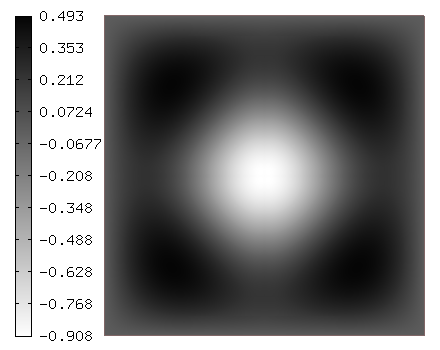
\includegraphics[width=0.4\textwidth]{img/eigen_5_ex.png}\ \ \ 
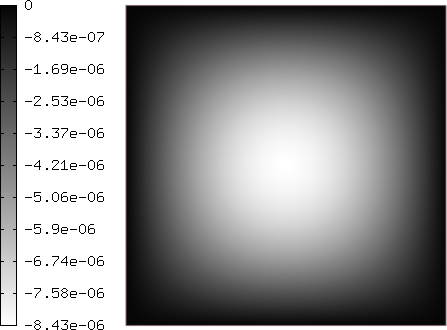
\includegraphics[width=0.433\textwidth]{img/eigen-new-1.png}
\end{center}
\vspace{-5mm}
\caption{The Picard's method converges from an initial guess that is very close to 
         the fifth eigenfunction (left) that corresponds to $\lambda_5 = 10$ to the 
         first eigenfunction (right) that corresponds to $\lambda_1 = 2$.}
\label{fig:picard}
\end{figure}

%%%%%%%%%%%%%%%%%%%%%%%%%%%%%%%%%%%%%%%%%%%%%%%%%%%%%%%%%%%%%%%%%%%%%%%%%%%%%%%%%%%%%%%%%%%%%%%%%%%%%%%%%

\section{Picard's Method with Orthogonalization}\label{sec:picard++}

In order to make the Picard's method suitable to approximate efficiently any discrete eigenpair, and not only the first one, we derived Algorithm~\ref{alg:picard_ortho}, which has an orthogonalization procedure in it.

The Picard's method with orthogonalization takes as arguments the matrices $\mathbf{A}$ and $\mathbf{B}$ of \eqref{eq:disc_prob}, an initial guess $\tilde u$ for the eigenfunction, a tolerance $\mathrm{Tol}$ and it also takes the $j-1$ eigenfunctions $u_{1,n},\dots,u_{j-1,n}$.
Then it returns the eigenpair $\lambda_{j,n},u_{j,n}$. 
Then it returns the eigenpair $\lambda_{j,n},u_{j,n}$ on the refined mesh.

%{\red STEFANO, do you want to move the following statement after the Algorithm, 
%and formulate it as a Theorem with 
%a simple proof? To me this would look stronger.}

%This method never converges to an eigenfunction of index smaller than $j$ because for any $m\ge 1$, the vector $\mathbf{u}^m$ is orthogonal to all eigenfunctions $u_{1,n},\dots,u_{j-1,n}$, i.e. all coefficients 
%$c_1^m,\dots,c_{j-1}^m$ in the expansion of $\mathbf{u}^m$ are zero, so the eigenvalue smallest in module is $\lambda_j$ and the Picard's method naturally converges to it.

%Anyway this is not enough to guarantee to not lose the eigenfunction that we want because if a multiple eigenspace splits differently due to the refinement of the mesh, the eigenfunction of the refined mesh are not similar to the wanted eigenfunction on the coarse mesh.

%\textcolor{red}{Pavel, we should try to find such an example.}

\begin{algorithm}[H] \caption{Picard's method with orthogonalization} \label{alg:picard_ortho} 
\begin{algorithmic}

\STATE{$(\lambda_{j,n},u_{j,n}):=\mathrm{PicardOrtho}
    (\mathbf{A}, \mathbf{B},\tilde u_{j,n-1},\mathrm{Tol},\mathrm{AbsTol},u_{1,n},\dots
    ,u_{j-1,n})$}
    

\STATE{$\mathbf{u}^1:=\tilde u_{j,n-1}$}
\STATE{$\displaystyle\lambda^{1}:=\frac{u_{j,n}^t\mathbf{A}u_{j,n}}{u_{j,n}^t\mathbf{B}u_{j,n}}$}
\STATE{$m=1$}
\REPEAT

\STATE{$\mathbf{u}^{m+1}:=\mathbf{A}^{-1}\lambda^m\mathbf{B}\mathbf{u}^{m}$}


\FOR{$i = 1$ to $j-1$} 
\STATE $\mathbf{u}^{m+1}:=\mathbf{u}^{m+1}-(u_{i,n}^t\mathbf{B}\mathbf{u}^{m+1})u_{i,n}$
\COMMENT{Orthogonalization}
\ENDFOR


\STATE $\displaystyle \mathbf{u}^{m+1}=\frac{\mathbf{u}^{m+1}}{((\mathbf{u}^{m+1})^t\mathbf{B}\mathbf{u}^{m+1})^{1/2}}$
\COMMENT{Normalize}
\STATE{$\displaystyle\lambda^{m+1}:=\frac{(\mathbf{u}^{m+1})^t\mathbf{A}\mathbf{u}^{m+1}}{(\mathbf{u}^{m+1})^t\mathbf{B}\mathbf{u}^{m+1}}$}
\STATE{$m:=m+1$}
\UNTIL{ $\frac{\|\mathbf{u}^{m+1}-\mathbf{u}^{m}\|_1}{\|\mathbf{u}^{m}\|_1}>\mathrm{Tol}$ \bf{and}
$|\lambda^{m+1}-\lambda^m|>\mathrm{AbsTol}$}
\STATE{$u_{j,n}:=\mathbf{u}^{m}$}
\STATE{$\lambda_{j,n}:=\lambda^m$}
\end{algorithmic}
\end{algorithm}

As can be seen in Algorithm~\ref{alg:picard_ortho}, the orthogonalization is done in each iteration. 
This is necessary in real arithmetic to guarantee that $\mathbf{u}^m$ is orthogonal to all 
eigenfunctions $u_{1,n},\dots,u_{j-1,n}$, for all $m$. Otherwise in exact arithmetic it would 
be enough to orthogonalize only $\mathbf{u}^1$. Moreover, a normalization step is necessary 
in all iterations because due to the orthogonalization procedure, this version of the Picard's 
method does not conserve the norm of the vectors and possible underflows or overflows could 
happen with no normalization.\\

\begin{theorem}
Algorithm~\ref{alg:picard_ortho} never converges to an eigenvalue of index smaller than $j$.
\end{theorem}

\begin{proof}
The proof comes straightforwardly from the arguments used to prove Theorem~\ref{th:picard_conv}.
The fact that $\mathbf{u}^m$ is orthogonal to all eigenfunctions $\mathbf{u}_1,\dots,\mathbf{u}_{j-1}$, implies that the coefficients $c_i^m$, with $m=1,\dots,j-1$, are zeros.
Then, the Rayleigh quotient converges to $\lambda_j$ by the same arguments use before.
\end{proof}



\noindent
{\bf Remark}: To make the Picard's method usable in practice, it is 
recommended to enhance it with Anderson acceleration \cite{anderson}.
This method combines a number of last iterates in a GMRES-like fashion. 
The result is equivalent to a Jacobian-free quasi-Newton (Broyden) method.

%%%%%%%%%%%%%%%%%%%%%%%%%%%%%%%%%%%%%%%%%%%%%%%%%%%%%%%%%%%%%%%%%%%%%%%%%%%%%%%%%%%%%%%%%%%%%%%%%%%%%%%%%

\section{Newton's Method with Orthogonalization}\label{sec:newton}

The second iterative method that we are going to propose is based on the Newton's method applied to eigenvalue problems. Denoting by $\tilde x:=(x,\lambda)$, we have that problem \eqref{eq:var_prob} can be rewritten in the form
$$
0=f(\tilde x):=
\left(
\begin{array}{lcl}
A x&-& \lambda_j\ Bx
\\
  x^T Bx&-& 1
\end{array}\quad
\right) ,
$$
then denoting by $\tilde h:=(h, \delta)$ the increment, we have that the truncated Taylor series of the problem is
\begin{equation}\label{eq:newton}
f(\tilde x + \tilde h)\approx f(\tilde x) + J_f(\tilde x)\cdot \tilde h, 
\end{equation}
where the Jacobian matrix is defined as
$$
J_f(\tilde x):=
\left(
\begin{array}{lr}
A - B\lambda & -Bx
\\
  2Bx^T  & 0
\end{array}\quad
\right) .
$$

Then when $\tilde x + \tilde h$ is a solution of \eqref{eq:var_prob}, we have from \eqref{eq:newton}
that 
$$
J_f(\tilde x)\cdot \tilde h = - f(\tilde x),
$$
which defines the linear problem of the Newton's method that we are solving.
\begin{algorithm}[H] \caption{Newton's method} \label{alg:newton} 
\begin{algorithmic}

\STATE{$(\lambda_{j,n},u_{j,n}):=\mathrm{Newton}
    (\mathbf{A}, \mathbf{B},\tilde u,\mathrm{Tol},\mathrm{AbsTol})$}

\STATE{$\mathbf{u}^1:=\tilde u$}
\STATE{$\displaystyle\lambda^{1}:=\frac{u_{j,n}^t\mathbf{A}u_{j,n}}{u_{j,n}^t\mathbf{B}u_{j,n}}$}
\STATE{$m=1$}
\REPEAT

\STATE{Solve $J_f(\mathbf{u}^m,\lambda^m)\cdot \tilde h = - f(\mathbf{u}^m,\lambda^m)$}
\STATE{$\mathbf{u}^{m+1}:=\mathbf{u}^m+h$}
\STATE{$\lambda^{m+1}:=\lambda^m+\delta$}
\STATE{$m:=m+1$}
\UNTIL{ $\frac{\|\mathbf{u}^{m+1}-\mathbf{u}^{m}\|_1}{\|\mathbf{u}^{m}\|_1}>\mathrm{Tol}$ \bf{and}
$|\lambda^{m+1}-\lambda^m|>\mathrm{AbsTol}$}
\STATE{$u_{n}:=\mathbf{u}^{m}$}
\STATE{$\lambda_{n}:=\lambda^m$}
\end{algorithmic}
\end{algorithm}

In order to make the method suitable for all eigenpairs, we are going write a version of the Newton's method that uses an orthogonalization procedure, similarly to what we have already done for the Picard's method.
\begin{algorithm}[H] \caption{Newton's method with orthogonalization} \label{alg:newton_ortho} 
\begin{algorithmic}

\STATE{$(\lambda_{j,n},u_{j,n}):=\mathrm{NewtonOrtho}
    (\mathbf{A}, \mathbf{B},\tilde u_{j,n-1},\mathrm{Tol},\mathrm{AbsTol},u_{1,n},\dots
    ,u_{j-1,n})$}
    

\STATE{$\mathbf{u}^1:=\tilde u_{j,n-1}$}
\STATE{$\displaystyle\lambda^{1}:=\frac{u_{j,n}^t\mathbf{A}u_{j,n}}{u_{j,n}^t\mathbf{B}u_{j,n}}$}
\STATE{$m=1$}
\REPEAT

%\STATE{$\mathbf{u}^{m+1}:=\mathbf{A}^{-1}\lambda^m\mathbf{B}\mathbf{u}^{m}$}
\STATE{Solve $J_f(\mathbf{u}^m,\lambda^m)\cdot h = - f(\mathbf{u}^m,\lambda^m)$}
\STATE{$\mathbf{u}^{m+1}:=\mathbf{u}^m+h$}
\STATE{$\lambda^{m+1}:=\lambda^m+\delta$}
\STATE{$m:=m+1$}


\FOR{$i = 1$ to $j-1$} 
\STATE $\mathbf{u}^{m+1}:=\mathbf{u}^{m+1}-(u_{i,n}^t\mathbf{B}\mathbf{u}^{m+1})u_{i,n}$
\COMMENT{Orthogonalization}
\ENDFOR


\STATE $\displaystyle \mathbf{u}^{m+1}:=\frac{\mathbf{u}^{m+1}}{((\mathbf{u}^{m+1})^t\mathbf{B}\mathbf{u}^{m+1})^{1/2}}$
\COMMENT{Normalize}
\STATE{$\displaystyle\lambda^{m+1}:=\frac{(\mathbf{u}^{m+1})^t\mathbf{A}\mathbf{u}^{m+1}}{(\mathbf{u}^{m+1})^t\mathbf{B}\mathbf{u}^{m+1}}$}
\STATE{$m:=m+1$}
\UNTIL{$\frac{\|\mathbf{u}^{m+1}-\mathbf{u}^{m}\|_1}{\|\mathbf{u}^{m}\|_1}>\mathrm{Tol}$ \bf{and}
$|\lambda^{m+1}-\lambda^m|>\mathrm{AbsTol}$}
\STATE{$u_{j,n}:=\mathbf{u}^{m}$}
\STATE{$\lambda_{j,n}:=\lambda^m$}
\end{algorithmic}
\end{algorithm}

\begin{theorem}
Algorithm~\ref{alg:newton_ortho} converges always to an eigenvalue greater or equal to $\lambda_j$.
\end{theorem}

\begin{proof}
This result is a direct consequence of the orthogonalization step in Algorithm~\ref{alg:newton_ortho}.
We are using again the fact that any vector $\mathbf{u}^{m+1}$ can be expressed as 
$$
\mathbf{u}^{m+1}=\sum_{i=1}^N c_i^{m+1} \mathbf{u}_i,
$$
where $c_i^{m+1}$ are real coefficients, $N$ is the size of the matrices $\mathbf{A}$ and $\mathbf{B}$ and the vectors $\mathbf{u}_i\equiv u_{i,n}$ are the eigenvectors of the discrete problem, which are sorted accordingly the magnitude of the corresponding eigenvalues $\lambda_i$.
In particular, when $\mathbf{u}^{m+1}:=\mathbf{u}^m+h$, where $h$ is the solution of 
$J_f(\mathbf{u}^m,\lambda^m)\cdot h = - f(\mathbf{u}^m,\lambda^m)$, we have that, after the application of the orthogonalization step, the resulting vector is
$$
\mathbf{\hat u}^{m+1}=\sum_{i=j}^N c_i^{m+1} \mathbf{u}_i.
$$
Then, it is straightforward to see that the Rayleigh quotient
$$
\displaystyle\lambda^{m+1}:=\frac{(\mathbf{\hat u}^{m+1})^t\mathbf{A}\mathbf{\hat u}^{m+1}}{(\mathbf{\hat u}^{m+1})^t\mathbf{B}\mathbf{\hat u}^{m+1}} \ge \lambda_j.
$$
\end{proof}

%{\red STEFANO, it would be nice to have some sort of a Theorem with proof here, to 
%say something formal about the Newton's method with orthogonalization. Otherwise this 
%looks unfinished.}

%{\red Pavel, I'm working on it.}

%%%%%%%%%%%%%%%%%%%%%%%%%%%%%%%%%%%%%%%%%%%%%%%%%%%%%%%%%%%%%%%%%%%%%%%%%%%%%%%%%%%%%%%%%%%%%%%%%%%%%%%%%

\section{Automatic $hp$-Adaptivity}\label{sec:adapt}

With the Picard's and Newton's methods in hand, we can now proceed to automatic $hp$-adaptivity. 
We use an algorithm from \cite{solin3} that is an analogy to embedded higher-order ODE methods: 
In each adaptivity step it 
constructs an approximation pair with different orders of accuracy and uses their difference 
as an a-posteriori error estimator. 

Let $\cT^c_{0}$ be an initial coarse mesh. We construct an initial fine mesh $\cT^f_{0}$
by refining all elements in space and moreover increasing their polynomial degrees by one.
A generalized eigensolver is called one time only, 
to obtain a solution pair $(\lambda^c_{0}, u^c_{0})$
on the initial coarse mesh $\cT^c_{0}$. 

\begin{algorithm}[H] \caption{Automatic $hp$-Adaptivity} \label{alg:hp} 
\begin{algorithmic}
\STATE{Set $k := 0$}
\REPEAT
\STATE{Project the approximation $u^c_{k}$ to the mesh $\cT^f_{k}$. The projection 
       is denoted by $P^f_k u^c_{k}$. Since the finite element spaces on meshes 
       $\cT^c_{k}$ and $\cT^f_{k}$ are embedded, there is no projection error. }
\STATE{Calculate an initial guess $\tilde \lambda^f_{k}$ for the eigenvalue on the mesh $\cT^f_{k}$
       using the relation 
$$
  \tilde \lambda^f_{k} = \frac{(P^f_k u^c_{k})^T \mathbf{A}^f_{k} P^f_k u^c_{k}}{(P^f_k u^c_{k})^T 
  \mathbf{B}^f_{k} P^f_k u^c_{k}},
$$
where $\mathbf{A}^f_{k}$ and $\mathbf{B}^f_{k}$ are the stiffness and mass matrices on the 
mesh $\cT^f_{k}$, respectively.} 

The pair $(\tilde \lambda^f_{k}, P^f_k u^c_{k})$ is {\bf not a solution} to the generalized eigenproblem 
on the mesh $\cT^f_{k}$, but it is a good initial guess. 
\STATE{
Apply the Picard's or Newton's method as described in Sections \ref{sec:picard++} and \ref{sec:newton},
to obtain a solution pair $(\lambda^f_{k}, u^f_{k})$ on the mesh $\cT^f_{k}$.}
\STATE{
Project the approximation $u^f_{k}$ back to the coarse mesh 
$\cT^c_{k}$ to obtain $P^c_k u^f_{k}$. }
\STATE{
Calculate an a-posteriori error estimate $e^c_{k}$,
$$
  e^c_{k} = u^f_{k} - P^c_k u^f_{k}.
$$
Note: $e^c_{k}$ is a function, not a number.}
\STATE{
 Use $e^c_{k}$ to guide one step of automatic $hp$-adaptivity \cite{solin3} that 
 yields a new coarse mesh $\cT^f_{k+1}$.}
\STATE{Update $k := k+1$}
\UNTIL{The $H^1$-norm of $e^c_{k-1}$ is sufficiently small.}
\end{algorithmic}
\end{algorithm}

 

%%%%%%%%%%%%%%%%%%%%%%%%%%%%%%%%%%%%%%%%%%%%%%%%%%%%%%%%%%%%%%%%%%%%%%%%%%%%%%%%%%%%%%%%%%%%%%%%%%%%%%%%%


\section{Reconstruction Technology}\label{sec:reco}

It is well known that the discretization process perturbs the spectrum, in particular the eigenspace $E(\lambda_j)$ of multiple eigenvalue $\lambda_j$ can be split in more than one discrete eigenspace $E(\lambda_{j,n}),E(\lambda_{j+1,n}),\dots,E(\lambda_{j+m,n})$ with correspondent discrete eigenvalues $\lambda_{j,n},\lambda_{j+1,n},\dots,\lambda_{j+m,n}$ forming a small cluster for sufficiently rich finite element space, also under the same assumption we have that
$$
\mathrm{dim}\ E(\lambda_j)=\sum_{i=0}^m\mathrm{dim}\ E(\lambda_{j+i,n}).
$$
This phenomenon is already well documented in literature,  see \cite{strang, babuska, hackbusch}.

Different finite element spaces can split the same multiple eigenspace in different ways, this also happens with adaptively refined meshes. It is not rare that the same multiple eigenspace is split differently on the coarse and on the refined meshes. A different split corresponds to different discrete eigenfunctions, then it is not always possible to find for the same eigenvalue on the refined mesh an eigenfunction similar to the one on the coarse mesh.

%\textcolor{red}{Pavel, I think we need another figure here. It would be easy to see the phenomenon on unstructured meshes.}

We propose a way to always construct on a refined mesh, an approximation of the same eigenfunction as on the coarse mesh. The idea is based on the fact that for a sufficiently rich finite element space, the space $M_n(\lambda_j)=\mathrm{span}\{E(\lambda_{j,n}),E(\lambda_{j+1,n}),\dots E(\lambda_{j+m,n})\}$ is an approximation of the space $E(\lambda_j)$, see \cite{strang}. Let us denote the space $M_{n,1}(\lambda_j)$ as the subspace of $M_n(\lambda_j)$ of functions with unit norm in the $L^2$.
So for any function $U_{n-1}\in M_{n-1,1}(\lambda_j)$, we propose the function $U_{n}\in M_{n,1}(\lambda_j)$ that minimize the $\|U_{n-1}-U_{n}\|_{0,\Omega}$ as an approximation of $U_{n-1}$ on the refined mesh. For a sufficiently rich finite element space the minimizer is unique. By construction
\begin{equation}\label{eq:const}
U_n=\sum_{i=1}^{R} c_i \ u_{i,n},
\end{equation}
where $u_{1,n},u_{2,n},\dots,u_{R,n}$, with $R=\mathrm{dim}\ E(\lambda_j)$, are eigenfunctions of the discrete problem forming  an orthonormal basis for
$M_{n,1}$ and where the coefficients $c_i$ satisfy 
\begin{equation}\label{eq:cond_on_corf}
\sum_{i=1}^{R} c_i^2=1.
\end{equation}

From the definition of problem \eqref{eq:var_prob} we have that the reconstructed eigenvalue is defined as
$$
\Lambda_n=\frac{a(U_n,U_n)}{b(U_n,U_n)}.
$$

The couple $(\Lambda_n,U_n)$ is not a discrete eigenpair of problem \eqref{eq:var_prob} in general, in section~\ref{sse:pcf_priori} we prove that $(\Lambda_n,U_n)$ converges a priori at the same rate as any other discrete eigenpair of \eqref{eq:var_prob} to a continuous eigenpair.

%%%%%%%%%%%%%%%%%%%%%%%%%%%%%%%%%%%%%%%%%%%%%%%%%%%%%%%%%%%%%%%%%%%%%%%%%%%%%%%%%%%%%%%%%%%%%%%%%%%%%%%%%
\section{Computing Reference Solution via Reconstruction}\label{sec:recoref}

In this section we present two algorithms to compute approximations of eigenpairs. Each algorithm is based on a different method to compute the discrete spectrum, but all of them use the reconstruction technology to keep track of the eigenfunction of interest.

In all algorithms we are going to use call an iterative eigensolver with calling interface
$\{(\lambda_{j,n},u_{j,n})_{j=1}^{i}\}:=\mathrm{Eigensolver}(\mathbf{A},\mathbf{B},i,\mathrm{Tol},\mathrm{MaxIter})$, that computes the set of discrete eigenpairs $\{(\lambda_{j,n},u_{j,n})\}_{j=1}^{i}$ and where $\mathbf{A}$ is the stiffness matrix of the problem, $\mathbf{B}$ is the mass matrix of the problem  $i$ is the number of eigenpairs to compute, $\mathrm{Tol}$ is the requested tolerance for the eigenpairs and $\mathrm{MaxIter}$ is the maximum number of iterations. 


All algorithm we describe below are based on the reconstruction technology which is guided by two parameters: $\mathrm{DTE}$ and $\mathrm{FIE}$. The parameter $\mathrm{DTE}$ should be equal to the multiplicity of the continuous eigenvalue $\lambda$ that the user want to approximate. All the algorithm works also when $\mathrm{DTE}$ contains an upper bound of the multiplicity of $\lambda$, so in practise the multiplicity of the target eigenvalue is not necessary to be known exactly. The parameter $\mathrm{FIE}$ should be equal to the index $i$ of the first discrete eigenvalue on the initial mesh $\lambda_{i,0}$ that approximates $\lambda$. The reconstruction technology is described in Algorithm~\eqref{alg:reconstruction}.

\begin{algorithm}[H] \caption{Reconstruction algorithm} \label{alg:reconstruction} 
\begin{algorithmic}

\STATE{$(\Lambda_n,U_n):=\mathrm{Reconstruction}
    (\{(\lambda_{j,n},u_{j,n})\}_{j=\mathrm{FIE}}^{\mathrm{FIE}+\mathrm{DTE}},
(\Lambda_{n-1},U_{n-1}))$}

\STATE{Compute $\displaystyle (\Lambda_n,U_n):=\sum_{i=\mathrm{FIE}}^{\mathrm{FIE}+\mathrm{DTE}}
b(u_{i,n},U_{n-1})u_{i,n}$}

\STATE{$\displaystyle U_n:=\frac{U_n}{\sqrt{b(U_n,U_n)}}$}
\COMMENT{Normalize}
\STATE{$\Lambda_n:=a(U_n,U_n)$}

\end{algorithmic}
\end{algorithm}

The first method is based on the Picard's method. The only three parameters not yet defined are $M$ which is the maximum number of mesh adaptation requested, $0<\mathrm{FIE}\mathrm{TE}\leq\mathrm{FIE}+\mathrm{DTE} $ which is the index of the eigenvalue that the user want to target and $\mathrm{err}$ which is tolerance for the residual.


\begin{algorithm}[H] \caption{Adaptive method based on the Picard's method} \label{alg:picard_adapt} 
\begin{algorithmic}

\STATE{$(\Lambda_M,U_M):=\mathrm{PicardAdapt}
    (\mathcal{T}_0, V_0,M,\mathrm{err},\mathrm{Tol},\mathrm{AbsTol},\mathrm{MaxIter}
,\mathrm{DTE},\mathrm{FIE},\mathrm{TE})$}

\STATE{Construct $\mathbf{A}_0$ and $\mathbf{B}_0$}

\STATE{$\{(\lambda_{j,0},u_{j,0})\}_{j=1}^{\mathrm{DTE}+\mathrm{FIE}}:=\mathrm{Eigensolver}(\mathbf{A}_0,\mathbf{B}_0,
\mathrm{DTE}+\mathrm{FIE},$}
\STATE{$\quad\quad\quad\mathrm{Tol},\mathrm{MaxIter})$}
\STATE{$(\Lambda_0,U_0):=(\lambda_{\mathrm{TE},0},u_{\mathrm{TE},0})$}
%\STATE{Compute the residual $\eta$ for the couple $(\Lambda_0,U_0)$}
\STATE{$m:=1$}
\REPEAT
\STATE{Construct $\mathbf{A}_m$ and $\mathbf{B}_m$}
\STATE{Construct the mesh $\mathcal{T}_m$ and the finite element space $V_m$ adapting $\mathcal{T}_{m-1}$ and $V_{m-1}$}
\STATE{$(\lambda_{1,m},u_{1,m}):=\mathrm{Picard}
    (\mathbf{A}_m, \mathbf{B}_m,u_{1,m-1},\mathrm{Tol},\mathrm{AbsTol})$}
\STATE{$j=1$}
\FOR{$j = 2$ to $\mathrm{DTE}+\mathrm{FIE}$}

\STATE{$(\lambda_{j,m},u_{j,m}):=\mathrm{PicardOrtho}
    (\mathbf{A}_m, \mathbf{B}_m,u_{j,m-1},\mathrm{Tol},\mathrm{AbsTol},u_{j,m-1},\dots
    ,u_{j-1,m-1})$}


\ENDFOR
\STATE{$(\Lambda_m,U_m):=\mathrm{Reconstruction}
    (\{(\lambda_{j,m},u_{j,m})\}_{j=\mathrm{FIE}}^{\mathrm{FIE}+\mathrm{DTE}},
(\Lambda_{m-1},U_{m-1}))$}
\STATE{Compute the residual $\eta$ for the couple $(\Lambda_m,U_m)$}
\STATE{$m:=m+1$}
\UNTIL{ $m\leq M$ OR $\eta \leq \mathrm{err}$}
\end{algorithmic}
\end{algorithm}

Similarly we define the adaptive method based on the Newton's method.

\begin{algorithm}[H] \caption{Adaptive method based on the Newton's method} \label{alg:newton_adapt} 
\begin{algorithmic}

\STATE{$(\Lambda_M,U_M):=\mathrm{NewtonAdapt}
    (\mathcal{T}_0, V_0,M,\mathrm{err},\mathrm{Tol},\mathrm{AbsTol},\mathrm{MaxIter}
,\mathrm{DTE},\mathrm{FIE},\mathrm{TE})$}

\STATE{Construct $\mathbf{A}_0$ and $\mathbf{B}_0$}

\STATE{$\{(\lambda_{j,0},u_{j,0})\}_{j=1}^{\mathrm{DTE}+\mathrm{FIE}}:=\mathrm{Eigensolver}(\mathbf{A}_0,\mathbf{B}_0,
\mathrm{DTE}+\mathrm{FIE},$}
\STATE{$\quad\quad\quad\mathrm{Tol},\mathrm{MaxIter})$}
\STATE{$(\Lambda_0,U_0):=(\lambda_{\mathrm{TE},0},u_{\mathrm{TE},0})$}
%\STATE{Compute the residual $\eta$ for the couple $(\Lambda_0,U_0)$}
\STATE{$m:=1$}
\REPEAT
\STATE{Construct $\mathbf{A}_m$ and $\mathbf{B}_m$}
\STATE{Construct the mesh $\mathcal{T}_m$ and the finite element space $V_m$ adapting $\mathcal{T}_{m-1}$ and $V_{m-1}$}
\STATE{$(\lambda_{1,m},u_{1,m}):=\mathrm{Newton}
    (\mathbf{A}_m, \mathbf{B}_m,u_{1,m-1},\mathrm{Tol},\mathrm{AbsTol})$}
\STATE{$j=1$}
\FOR{$j = 2$ to $\mathrm{DTE}+\mathrm{FIE}$}

\STATE{$(\lambda_{j,m},u_{j,m}):=\mathrm{NewtonOrtho}
    (\mathbf{A}_m, \mathbf{B}_m,u_{j,m-1},\mathrm{Tol},\mathrm{AbsTol},u_{1,m-1},\dots
    ,u_{j-1,m-1})$}


\ENDFOR
\STATE{$(\Lambda_m,U_m):=\mathrm{Reconstruction}
    (\{(\lambda_{j,m},u_{j,m})\}_{j=\mathrm{FIE}}^{\mathrm{FIE}+\mathrm{DTE}},
(\Lambda_{m-1},U_{m-1}))$}
\STATE{Compute the residual $\eta$ for the couple $(\Lambda_m,U_m)$}
\STATE{$m:=m+1$}
\UNTIL{ $m\leq M$ OR $\eta \leq \mathrm{err}$}
\end{algorithmic}
\end{algorithm}

%%%%%%%%%%%%%%%%%%%%%%%%%%%%%%%%%%%%%%%%%%%%%%%%%%%%%%%%%%%%%%%%%%%%%%%%%%%%%%%%%%%%%%%%%%%%%%%%%%%%%%%%%
\section{Iterative methods with improved orthogonalization}\label{sec:imp_ortho}

The main disadvantage of the algorithms presented in Sections~\ref{sec:picard++} and \ref{sec:newton} is the cost of the method. Those methods ensure that the eigenpair with the correct index $m$ is computed, but, in order to ensure that, all eigenpairs of indices from 1 to $n-1$ are also computed. What we present now is a more cheaper way to ensure the computation of the target eigenpair. The key idea is a smarter way to use the orthogonalization only when it is really necessary and this is possible mainly because we can use information from the previous mesh to identify unwanted eigenpairs.

The reason why we introduce the algorithms in Sections~\ref{sec:picard++} and \ref{sec:newton} was to cure the downside of the iterative methods to possibly converge to an eigenpair different from the target one. The answer to this problem presented in Sections~\ref{sec:picard++} and \ref{sec:newton} was to compute all possible eigenpair to which the method could erroneously converge to, and then use all of them to force the method using the orthogonalization to produce an approximation of the wanted eigenpair. There is a better method which consists in starting with no-orthogonalization and then every time that the iterative method produces an unwanted eigenpair, save it to be used next time in the orthogonalization process to prevent the method to converge again to the same unwanted solution. This is possible only if a way to distinguish between wanted and unwanted solution is available. In the adaptive setting this is always possible because  the orthogonality of any newly computed eigenpair against the results on the previous mesh can be computed.

The Algorithms~\ref{alg:picard_importho} and \ref{alg:newton_importho} are the incarnations of the improved orthogonality technology applied with the either the Picard's or the Newton's method respectively. Since these two algorithms are identical except for the call to either $\mathrm{PicardOrtho}$ or to $\mathrm{PicardOrtho}$, in the rest w are gong to describe only Algorithm~\ref{alg:picard_importho}.

Algorithm~\ref{alg:picard_importho} compute a set of eigenpairs $\{(\lambda_{j,n},u_{j,n})\}_{j=\mathrm{FIE}}^{\mathrm{DTE}+\mathrm{FIE}}$, approximating the target continuous eigenspace, on the mesh $\cT_n$. The arguments that it needs are: the matrices $\mathbf{A}$ and $\mathbf{B}$, the approximation of the target eigenspace $\{(\tilde\lambda_{j,n-1},\tilde u_{j,n-1})\}_{j=\mathrm{FIE}}^{\mathrm{DTE}+\mathrm{FIE}}$ computed on the previous mesh $\cT_{n-1}$, and then projected on the refined mesh $\cT_n$, and a real value $0<\mathrm{ThO}<1$ which is used to decide wether a computed eigenfunction is part of the approximation of the target eigenspace or not. The set $\mathcal{D}$ is empty at the beginning, but then it is fed with all computed eigenfunctions. Then $\mathcal{D}$ is passed to every call to $\mathrm{PicardOrtho}$ and so it guarantees that the same eigenfunction is never computed twice.
The key part of the algorithm is just after the call to $\mathrm{PicardOrtho}$, where the newly computed eigenfunction is analyzed. The analysis consists in checking how orthogonal the newly computed eigenfunction $u_{j,n}$ is respect to the span of $\{(\tilde\lambda_{j,n-1},\tilde u_{j,n-1})\}_{j=\mathrm{FIE}}^{\mathrm{DTE}+\mathrm{FIE}}$. If the resulting value is smaller than $\mathrm{ThO}$, then $u_{j,n}$ is not considered part of the target eigenspace and a new approximation of  $u_{j,n}$ is done. Otherwise, $u_{j,n}$ is kept and the algorithm pass to approximate the next eigenfunction in the target eigenspace.
The algorithm end when all eigenpair in $\{(\lambda_{j,n},u_{j,n})\}_{j=\mathrm{FIE}}^{\mathrm{DTE}+\mathrm{FIE}}$ are computed.

\begin{algorithm}[H] \caption{Picard's method with improved orthogonalization} \label{alg:picard_importho} 
\begin{algorithmic}

\STATE{$\{(\lambda_{j,n},u_{j,n})\}_{j=\mathrm{FIE}}^{\mathrm{DTE}+\mathrm{FIE}}:=\mathrm{PicardImpOrtho}
    (\mathbf{A}, \mathbf{B},\{(\tilde\lambda_{j,n-1},\tilde u_{j,n-1})\}_{j=\mathrm{FIE}}^{\mathrm{DTE}+\mathrm{FIE}},\mathrm{ThO})$}
\STATE{$\mathcal{D}:=\O$}
%\STATE{$m:=1$}
\STATE{$j:=\mathrm{DTE}+\mathrm{FIE}$}
\REPEAT
\STATE{$(\lambda_{j,n},u_{j,n}):=\mathrm{PicardOrtho}
    (\mathbf{A}, \mathbf{B},u_{j,n-1},\mathrm{Tol},\mathrm{AbsTol},\mathcal{D})$}
    %\STATE{$m:=m+1$}
    \STATE{Add $u_{j,n}$ to $\mathcal{D}$}
    \STATE{$\mathrm{inner}:=0$}
    \FOR{$i = \mathrm{FIE} \to \mathrm{DTE}+\mathrm{FIE}$}
        \STATE{$\mathrm{inner}:=\mathrm{inner}+u_{j,n}^t\mathbf{B}\tilde u_{i,n-1}$}
    \ENDFOR
    \IF {$\mathrm{inner}>\mathrm{ThO}$}
       \STATE{$j:=j-1$}
    \ENDIF
\UNTIL{ $j<\mathrm{FIE}$}% OR $m>\mathrm{DTE}+\mathrm{FIE}$}
\end{algorithmic}
\end{algorithm}

\begin{algorithm}[H] \caption{Newton's method with improved orthogonalization} \label{alg:newton_importho} 
\begin{algorithmic}

\STATE{$\{(\lambda_{j,n},u_{j,n})\}_{j=\mathrm{FIE}}^{\mathrm{DTE}+\mathrm{FIE}}:=\mathrm{NewtonImpOrtho}
    (\mathbf{A}, \mathbf{B},\{(\tilde\lambda_{j,n-1},\tilde u_{j,n-1})\}_{j=\mathrm{FIE}}^{\mathrm{DTE}+\mathrm{FIE}},\mathrm{ThO})$}
\STATE{$\mathcal{D}:=\O$}
%\STATE{$m:=1$}
\STATE{$j:=\mathrm{DTE}+\mathrm{FIE}$}
\REPEAT
\STATE{$(\lambda_{j,n},u_{j,n}):=\mathrm{NewtonOrtho}
    (\mathbf{A}, \mathbf{B},u_{j,n-1},\mathrm{Tol},\mathrm{AbsTol},\mathcal{D})$}
    %\STATE{$m:=m+1$}
    \STATE{Add $u_{j,n}$ to $\mathcal{D}$}
    \STATE{$\mathrm{inner}:=0$}
    \FOR{$i = \mathrm{FIE} \to \mathrm{DTE}+\mathrm{FIE}$}
        \STATE{$\mathrm{inner}:=\mathrm{inner}+u_{j,n}^t\mathbf{B}\tilde u_{i,n-1}$}
    \ENDFOR
    \IF {$\mathrm{inner}>\mathrm{ThO}$}
       \STATE{$j:=j-1$}
    \ENDIF
\UNTIL{ $j<\mathrm{FIE}$}% OR $m>\mathrm{DTE}+\mathrm{FIE}$}
\end{algorithmic}
\end{algorithm}

So the number of computed eigenfunction may vary: in the best case scenario when the method is used to approximate an eigenspace of dimension $\mathrm{DTE}$, only $\mathrm{DTE}$ eigenfunctions are computed. In the worst case scenario, $\mathrm{DTE}+\mathrm{FIE}$ eigenfunctions are computed, which is the number of computed eigenfunctions by Algorithms~\ref{alg:picard_ortho},~\ref{alg:newton_ortho} on the same space. Because almost never the worst case scenario is achieved, Algorithms~\ref{alg:picard_importho} and \ref{alg:newton_importho} are more efficient than Algorithms~\ref{alg:picard_ortho},~\ref{alg:newton_ortho}.

We conclude this section stating the adaptive algorithms with improved orthogonality.

\begin{algorithm}[H] \caption{Adaptive method based on the Picard's method with improved orthogonality} \label{alg:picard_impadapt} 
\begin{algorithmic}

\STATE{$(\Lambda_M,U_M):=\mathrm{PicardImpAdapt}
    (\mathcal{T}_0, V_0,M,\mathrm{err},\mathrm{Tol},\mathrm{MaxIter}
,\mathrm{DTE},\mathrm{FIE},\mathrm{TE},\mathrm{ThO})$}

\STATE{Construct $\mathbf{A}_0$ and $\mathbf{B}_0$}

\STATE{$\{(\lambda_{j,0},u_{j,0})\}_{j=1}^{\mathrm{DTE}+\mathrm{FIE}}:=\mathrm{Eigensolver}(\mathbf{A}_0,\mathbf{B}_0,
\mathrm{DTE}+\mathrm{FIE},$}
\STATE{$\quad\quad\quad\mathrm{Tol},\mathrm{MaxIter})$}
\STATE{$(\Lambda_0,U_0):=(\lambda_{\mathrm{TE},0},u_{\mathrm{TE},0})$}
%\STATE{Compute the residual $\eta$ for the couple $(\Lambda_0,U_0)$}
\STATE{$m:=1$}
\REPEAT
\STATE{Construct $\mathbf{A}_m$ and $\mathbf{B}_m$}
\STATE{Construct the mesh $\mathcal{T}_m$ and the finite element space $V_m$ adapting $\mathcal{T}_{m-1}$ and $V_{m-1}$}
\STATE{$\{(\lambda_{j,m},u_{j,m})\}_{j=\mathrm{FIE}}^{\mathrm{DTE}+\mathrm{FIE}}:=\mathrm{PicardImpOrtho}
    (\mathbf{A}_m, \mathbf{B}_m,\{(\lambda_{j,m-1}, u_{j,m-1})\}_{j=\mathrm{FIE}}^{\mathrm{DTE}+\mathrm{FIE}},\mathrm{ThO})$}

\STATE{$(\Lambda_m,U_m):=\mathrm{Reconstruction}
    (\{(\lambda_{j,m},u_{j,m})\}_{j=\mathrm{FIE}}^{\mathrm{FIE}+\mathrm{DTE}},
(\Lambda_{m-1},U_{m-1}))$}
\STATE{Compute the residual $\eta$ for the couple $(\Lambda_m,U_m)$}
\STATE{$m:=m+1$}
\UNTIL{ $m\leq M$ OR $\eta \leq \mathrm{err}$}
\end{algorithmic}
\end{algorithm}

Similarly we define the adaptive method based on the Newton's method.

\begin{algorithm}[H] \caption{Adaptive method based on the Newton's method with improved orthogonality} \label{alg:newton_impadapt} 
\begin{algorithmic}

\STATE{$(\Lambda_M,U_M):=\mathrm{PicardImpAdapt}
    (\mathcal{T}_0, V_0,M,\mathrm{err},\mathrm{Tol},\mathrm{MaxIter}
,\mathrm{DTE},\mathrm{FIE},\mathrm{TE},\mathrm{ThO})$}

\STATE{Construct $\mathbf{A}_0$ and $\mathbf{B}_0$}

\STATE{$\{(\lambda_{j,0},u_{j,0})\}_{j=1}^{\mathrm{DTE}+\mathrm{FIE}}:=\mathrm{Eigensolver}(\mathbf{A}_0,\mathbf{B}_0,
\mathrm{DTE}+\mathrm{FIE},$}
\STATE{$\quad\quad\quad\mathrm{Tol},\mathrm{MaxIter})$}
\STATE{$(\Lambda_0,U_0):=(\lambda_{\mathrm{TE},0},u_{\mathrm{TE},0})$}
%\STATE{Compute the residual $\eta$ for the couple $(\Lambda_0,U_0)$}
\STATE{$m:=1$}
\REPEAT
\STATE{Construct $\mathbf{A}_m$ and $\mathbf{B}_m$}
\STATE{Construct the mesh $\mathcal{T}_m$ and the finite element space $V_m$ adapting $\mathcal{T}_{m-1}$ and $V_{m-1}$}
\STATE{$\{(\lambda_{j,m},u_{j,m})\}_{j=\mathrm{FIE}}^{\mathrm{DTE}+\mathrm{FIE}}:=\mathrm{NewtonImpOrtho}
    (\mathbf{A}_m, \mathbf{B}_m,\{(\lambda_{j,m-1}, u_{j,m-1})\}_{j=\mathrm{FIE}}^{\mathrm{DTE}+\mathrm{FIE}},\mathrm{ThO})$}

\STATE{$(\Lambda_m,U_m):=\mathrm{Reconstruction}
    (\{(\lambda_{j,m},u_{j,m})\}_{j=\mathrm{FIE}}^{\mathrm{FIE}+\mathrm{DTE}},
(\Lambda_{m-1},U_{m-1}))$}
\STATE{Compute the residual $\eta$ for the couple $(\Lambda_m,U_m)$}
\STATE{$m:=m+1$}
\UNTIL{ $m\leq M$ OR $\eta \leq \mathrm{err}$}

\end{algorithmic}
\end{algorithm}

%%%%%%%%%%%%%%%%%%%%%%%%%%%%%%%%%%%%%%%%%%%%%%%%%%%%%%%%%%%%%%%%%%%%%%%%%%%%%%%%%%%%%%%%%%%%%%%%%%%%%%%%%
\section{A Priori Convergence Results}\label{sse:pcf_priori}\label{sec:aprio}

%\textcolor{red}{This section is for smooth problems only, i.e. $u\in H^s(\Omega)$, $s\ge 2$.}

In this section  we gather together some a priori estimates for eigenvalue
problems.  The framework used in this section is an extension to the $hp-$case of the a priori results in 
\cite{giani1,pcf_apost}. Lemma~\ref{lm:adj} contains the a priori convergence results for eigenvalues and eigenfunctions in the $hp$ context. Moreover, in Theorem~\ref{th:adj_rec} we proved convergence a priori results for the reconstructed eigenpair $(\Lambda_n,U_n)$.




It follows from the coercivity of the bilinear form $a(\cdot,\cdot)$ that
all eigenvalues of  \eqref{eq:var_prob} and all $N=\dim V_n$
eigenvalues of \eqref{eq:disc_prob} are positive.
We can order
them as $0 < \lambda_1 \leq \lambda_2 \ldots $ and $0 < \lambda_{1,n}
\leq \lambda_{2,n} \ldots \leq \lambda_{N,n}$. Moreover, we know (e.g. 
\cite{BaOs:89}) that  $\lambda_{j,n} \rightarrow \lambda_j$,
for any
$j$,  as  $V_n
\rightarrow H^1(\Omega)$ and (by the minimax principle) 
that $\lambda_{j,n}$ is monotone
non-increasing, i.e.
\begin{equation}\label{eq:minimax_shift}
\lambda_{j,n} \ \geq\  \lambda_{j,m}\  \geq\   \lambda_j , \quad
\text{for all} \quad j = 1, \ldots , N, \quad \text{and all} \quad
m \geq n .
\end{equation}

The distance of an approximate eigenfunction from the true eigenspace
is a crucial quantity in the convergence analysis for
eigenvalue problems  especially in the case of non-simple
eigenvalues.

\begin{definition}
\label{def:dist_l2}
Given a function $v\in L^2(\Omega)$ and a finite dimensional subspace $\mathcal{P}\subset L^2(\Omega)$, we define:
$$
\mathrm{dist}(v,\mathcal{P})_{0,\cB}\ :=\ \min_{ w\in\mathcal{P}}  \|v-w\|_{0} .
$$
Similarly, given a function $v\in H^1_\pi(\Omega)$ and a finite dimensional subspace $\mathcal{P}\subset H^1_\pi(\Omega)$, we define:
$$
\mathrm{dist}(v,\mathcal{P})_{1}\ :=\ \min_{ w\in\mathcal{P}}  \|v-w\|_{1} .
$$
\end{definition}

Now let $\lambda_j$ be any eigenvalue of 
\eqref{eq:var_prob},  let $E(\lambda_j)$ denote the (finite
dimensional) space spanned by  the eigenfunctions of  $\lambda_j$ and set
$E_1(\lambda_j)=\{u\in E(\lambda_j):
\|u\|_{0}=1\}$. 
{Let $T_{\lambda_j}$
  denote the orthogonal projection of $H^1$ onto $E(\lambda_j)$ with respect
  to the inner product $a(\cdot, \cdot)$.}

The next lemma is already in \cite{pcf_apost} and it shows that both distances have the same minimizer.


%%%%%%%%%%%%%%%%%%%%%%%%%%%%%%%%%%%%%%%%%%%%%%%%%%%%%%%%%%%%%%%%%%%%%%%%%%%%%%%%%%%%%%%%%%%%%%%%%%%%%%%%%
\begin{lemma}\label{lm:inf_l2_h1}
 Let $(\lambda_{j,n},u_{j,n})$ be an eigenpair of \eqref{eq:disc_prob}. Then
\begin{equation}\label{eq:inf_l2_h1_1}
\|u_{j,n}-u_j\|_{0} = \mathrm{dist}(u_{j,n},E_1(\lambda_j))_{0},
\end{equation}
if and only if
\begin{equation}\label{eq:inf_l2_h1_2}
\|{u_{j,n}-u_j}\|_{1}=\mathrm{dist}(u_{j,n},E_1(\lambda_j))_{1}.
\end{equation}

\end{lemma}

%\begin{proof}
%%\ednote{It is shortened - please read it carefully}
%{Since $E(\lambda_j)$ is
%finite dimensional,   
%the minimizers in \eqref{eq:inf_l2_h1_1} and \eqref{eq:inf_l2_h1_2}
%exist. Moreover 
%\begin{equation}\label{eq:l2_ortho_1}
%0  \ = \ a(T_{\lambda_j} w, (I-T_{\lambda_j}) v) \ =\
%\lambda_j\ b(T_{\lambda_j} w, (I-T_{\lambda_j}) v) \   \quad \text{for all} \quad 
%v,w\in L^2(\Omega)\cap H^1(\Omega)\ .
%\end{equation}
%Hence for any $v_j \in E(\lambda_j)$ we have the decomposition   
%$$u_{j,n}-v_j\ = \ (I-T_{\lambda_j})u_{j,n}\ +\ T_{\lambda_j} (u_{j,n}-v_j)
%\ = \  (I-T_{\lambda_j})u_{j,n}\ +\ (T_{\lambda_j} u_{j,n}-v_j) ,
%$$
%which is orthogonal both with respect to $a(\cdot, \cdot)$
%and $b(\cdot, \cdot)$. Thus 
%\begin{eqnarray*}
%\|u_{j,n}-v_j\|_{0}^2\ & = & \ 
%\|(I-T_{\lambda_j})u_{j,n}\|_{0}^2 +
%\|T_{\lambda_j} u_{j,n}-v_j\|_{0}^2,\\
%\|u_{j,n}-v_j\|_{1}^2\ & = & \ 
%\|(I-T_{\lambda_j})u_{j,n}\|_{1}^2 +
%\|T_{\lambda_j} u_{j,n}-v_j\|_{1}^2 .
%\end{eqnarray*}
%Hence $u_j$  satisfies \eqref{eq:inf_l2_h1_2}  if and only if it minimizes 
%$\|T_{\lambda_j}u_{j,n}-v_j\|_{1}^2$.  The latter quantity is
%equal to \\$\lambda_j \|T_{\lambda_j}u_{j,n}-v_j\|_{0}^2$
%and hence $u_j$ satisfies  \eqref{eq:inf_l2_h1_2} if and only
%if it satisfies \eqref{eq:inf_l2_h1_1}.}

%\end{proof}

%Let $u_j$ and $u_{j,n}$ be any
%normalized eigenvectors of \eqref{eq:var_prob}
%and \eqref{eq:disc_prob}.
%Then
%\begin{eqnarray}
%\label{eq:basic1} a(u_j - u_{j,n}, u_j - u_{j,n}) &=& a(u_j,u_j) +
%a(u_{j,n},u_{j,n})
%- 2 a(u_{j},u_{j,n})\nonumber\\
%&=&    \lambda_j +  \lambda_{j,n} -  2\lambda_j \ b(u_{j},u_{j,n})
%\nonumber\\
%&=&      (\lambda_{j,n} - \lambda_j)  +2  \lambda_j\ (1-b(u_{j},u_{j,n}))\nonumber\\
%&=&
%(\lambda_{j,n} - \lambda_j)  +\lambda_j\
%b(u_{j}-u_{j,n},u_{j}-u_{j,n} ) .
%\end{eqnarray}
%Combining this with \eqref{eq:minimax_shift}, we obtain
%\begin{equation}
%a(u_j-u_{j,n},u_j-u_{j,n}) \ =\ |a(u_j-u_{j,n},u_j-u_{j,n})|\ =\  |\lambda_j-\lambda_{j,n}| \ + \
%\lambda_j \ \Vert u_{j}-u_{j,n}\Vert_{0,\cB}^2.
%\label{eq:basic2}
%\end{equation}

In order to make further progress we need some assumption on
regularity of solutions of elliptic problems associated with $a(\cdot,
\cdot)$. Also from now on we assume that the eigenfunctions of \eqref{eq:var_prob} are at least in $H^2(\Omega)$ and that the sequence of adapted meshes are at most 1-irregular.
%\textcolor{red}{If we are going to consider non-smooth problems, I need to change this assumption.}
\begin{assumption}\label{ass:ell}
 We assume that there exists a constant
$C_\mathrm{ell}>0$ with the following property.
For   $f \in L^2(\Omega)$ and with the solution operator $\cS$, we have that if  $v: = \cS f\in H^1_0(\Omega)$ solves  the
problem {$a(v,w) = b(f,w) $} for all $w \in
H^1_0(\Omega)$, then 
\begin{equation}\label{eq:ass_reg_pcf}
\Vert \cS f \Vert_{{2}} \leq
C_\mathrm{ell}\Vert f \Vert_0,
\end{equation}
where  $\Vert \cdot \Vert_{2}$ is the norm in   the Sobolev space $H^{2}(\Omega)$.
%\begin{equation}\label{eq:ass_reg_pcf}
%\Vert \mathcal{S} f \Vert_{{1+s}} \leq
%C_\mathrm{ell}\Vert f \Vert_0,
%\end{equation}
%where  $\Vert \cdot \Vert_{{1+s}}$ is the norm in   the Sobolev space $H^{1+s}(\Omega)$.
\end{assumption}
This is a standard assumption which is satisfied in a wide number of
applications such as problems with discontinuous coefficients
(see eg. \cite{conv_sinum} for more references).\\

From now on we shall let $C$ denote  a generic constant which 
may depend
on the 
true eigenvalues and vectors of \eqref{eq:var_prob} and other
constants introduced above, but is always independent of
$n$.  The next lemma is an extension of Theorem~3.5 in \cite{pcf_apost} based on the same arguments
and where $hp-$results like \cite[Theorem~4.72]{schwab} are used.



%%%%%%%%%%%%%%%%%%%%%%%%%%%%%%%%%%%%%%%%%%%%%%%%%%%%%%%%%%%%%%%%%%%%%%%%%%%%%%%%%%%%%%%%%%%%%%%%%%%%%%%%%
%\textcolor{red}{This theorem must be changed if we allow for non-smooth problems}
\begin{lemma}
\label{lm:adj}
Suppose  $ 1 \leq j\leq \dim V_n$. Let
$\lambda_j$ be an eigenvalue   of \eqref{eq:var_prob} with
corresponding eigenspace $E(\lambda_j)\subset H^{1+\mu}(\Omega)$, for $\mu>1$, of any (finite) dimension  and
let $(\lambda_{j,n},u_{j,n})$ be an  eigenpair  of \eqref{eq:disc_prob}.
Then, for a finite element space $V_n$ sufficiently rich,
\begin{itemize}
\item[(i)] 
\begin{equation}
\vert \lambda_j - \lambda_{j,n} \vert \ \leq \ (\mathrm{dist}(
u_{j,n},E_1(\lambda_j))_{1})^2; \quad \text{and} \quad
\vert \lambda_j - \lambda_{j,n} \vert \ \leq \ C
\frac{h_n^{2\mu} }{p_n^{2\mu}};  \label{eq:supereig}
\end{equation}
\item[(ii)] 
\begin{eqnarray}
\mathrm{dist}(
u_{j,n},E_1(\lambda_j))_{0}\ & \leq& \ C \frac{h_n}{p_n}
 \mathrm{dist}(
u_{j,n},E_1(\lambda_j))_{1} \ ; \label{eq:adj}
\end{eqnarray}
%\begin{eqnarray}
%\mathrm{dist}(
%u_{j,n},E_1(\lambda_j))_{0}\ & \leq& \ C \frac{h_n^s}{p_n^s}
% \mathrm{dist}(
%u_{j,n},E_1(\lambda_j))_{1} \ ; \label{eq:adj}
%\end{eqnarray}
\item[(iii)]
\begin{equation}
\label{eq:energy} \mathrm{dist}(
u_{j,n},E_1(\lambda_j))_{1} \ \leq
C \frac{h_n^{\mu}}{p_n^{\mu}}, 
\end{equation}
\end{itemize}
with $1\leq \mu\leq p_n$
\end{lemma}

%\begin{proof}\
%First consider part (i). 
%Since $\lambda_j \geq  0$, the first estimate in 
%\eqref{eq:supereig} follows directly from \eqref{eq:basic2}.
% To obtain the second estimate in \eqref{eq:supereig},  
%we recall a  standard error  estimate for elliptic eigenvalues   
%(see e.g.  \cite[(1.1)]{BaOs:89}) which gives  
%$$ \lambda_{j,n} - \lambda_j \ \leq \  C \sup_{u \in
%  E_1(\lambda_j)} \inf_{v_n \in V_n} \Vert u - v_n \Vert_1^2. $$
%Combining this with standard finite element error
%estimates for $hp$-method, see \cite[Theorem~4.72]{schwab} and 
%recalling \eqref{eq:minimax_shift}, we get  
%\begin{eqnarray}
%\vert \lambda_{j,n} - \lambda_j \vert \  \  
%\ \leq \ C \frac{h_n^{2\min(\mu,p)} }{p_n^{2\mu}} \sup_{u \in
%  E_1(\lambda_j)} \Vert u \Vert_{1+\mu}^2 ,  \label{eq:second_est} \end{eqnarray}
%% For  $u
%%\in E_1(\lambda_j)$, Assumption \ref{ass:ell} implies 
%%%$\Vert u \Vert_{1+s} \ \leq \ C_{ell} \lambda_j  \Vert u
%%%\Vert_{0}  \ \leq \ C_{ell} \lambda_j$
%%$\Vert u \Vert_2 \ \leq \ C_{ell} \lambda_j \Vert u
%%\Vert_{0}  \ \leq \ C_{ell} \lambda_j$,  which yields the
%%result. 

%To obtain  (ii),  we use the following estimate 
%\cite[(3.31a)]{BaOs:89}:
%\begin{equation}\label{eq:BaOs}\frac{\Vert T_{\lambda_j}u_{j, n} - u_{j, n}
%  \Vert_{0}}{\Vert T_{\lambda_j}u_{j, n} - u_{j, n}
%  \Vert_{1}} \ \leq \ C \eta_n, \quad 
%\text{where} \quad \eta_n \ = \ \sup_{\stackrel{g \in L^2(\Omega)}{\Vert
%    g\Vert_{0} = 1 }} \inf_{\chi \in V_n} \Vert \cS g - \chi
%\Vert_{1}, \end{equation} and $\cS $ is the solution
%operator defined in
%Assumption \ref{ass:ell}. Analogously to \eqref{eq:second_est} and with the further restriction that $\cS g\in H^2(\Omega)$ only, we have
%$\eta_n \leq C h_n p_n^{-1}$ and hence \eqref{eq:BaOs} implies
% \begin{eqnarray}
%\Vert T_{\lambda_j}u_{j, n} - u_{j, n}
%  \Vert_0 \ & \leq  & \  C     \frac{h_n}{p_n} \Vert T_{\lambda_j}u_{j, n} - u_{j, n}
%  \Vert_1  \nonumber \\
%& =  & \ C \frac{h_n}{p_n} \mathrm{dist} (u_{j,n}
%,E(\lambda_j))_1  \nonumber  \\ 
%& \leq & \  C   \frac{h_n}{p_n} \mathrm{dist} (u_{j,n}
%,E_1(\lambda_j))_1,  \label{eq:new2}
% \end{eqnarray} 
%%  \begin{eqnarray}
%%\Vert T_{\lambda_j}u_{j, n} - u_{j, n}
%%  \Vert_0 \ & \leq  & \  C     \frac{h_n^s}{p_n^{s-1}} \Vert T_{\lambda_j}u_{j, n} - u_{j, n}
%%  \Vert_1  \nonumber \\
%%& =  & \ C \frac{h_n^s}{p_n^{s-1}} \mathrm{dist} (u_{j,n}
%%,E(\lambda_j))_1  \nonumber  \\ 
%%& \leq & \  C   \frac{h_n^s}{p_n^{s-1}} \mathrm{dist} (u_{j,n}
%%,E_1(\lambda_j))_1 ,  \label{eq:new2}
%% \end{eqnarray} 
%where we used the inclusion $E_1(\lambda_j) \subset E(\lambda_j)$. 
%Since $\Vert u_{j,n}\Vert_0 = 1$,  \eqref{eq:new2} also implies
%that 
% \begin{eqnarray}
%\bigg\vert \Vert T_{\lambda_j}u_{j, n} \Vert_0  -1 \bigg\vert \
%& \leq  & \  \Vert T_{\lambda_j}u_{j, n} - u_{j, n}
%  \Vert_0  \nonumber  \\
%& \leq & \  C   \frac{h_n}{p_n} \mathrm{dist} (u_{j,n}
%,E_1(\lambda_j))_1 . \label{eq:new4}
% \end{eqnarray} 
%%  \begin{eqnarray}
%%\bigg\vert \Vert T_{\lambda_j}u_{j, n} \Vert_0  -1 \bigg\vert \
%%& \leq  & \  \Vert T_{\lambda_j}u_{j, n} - u_{j, n}
%%  \Vert_0  \nonumber  \\
%%& \leq & \  C   \frac{h_n^s}{p_n^{s-1}} \mathrm{dist} (u_{j,n}
%%,E_1(\lambda_j))_1 . \label{eq:new4}
%% \end{eqnarray} 
%Combining \eqref{eq:new2} and  \eqref{eq:new4},  we obtain
%\begin{eqnarray*} 
%\mathrm{dist}(u_{j,n}, E_1(\lambda_j))_0 \ & \leq & \ 
%\bigg\Vert \frac{T_{\lambda_j}u_{j, n}}{\Vert T_{\lambda_j}u_{j, n}\Vert_0} - u_{j, n}
%  \bigg\Vert_0 \\
%& \leq & \ 
%\bigg\Vert {T_{\lambda_j}u_{j, n}} - u_{j, n}
%  \bigg\Vert_0 + \bigg\vert 1 - \Vert T_{\lambda_j}u_{j,n}\Vert_0^{-1}\bigg\vert  \ \Vert T_{\lambda_j}u_{j,n}\Vert_0\\
%& =  & \ 
%\bigg\Vert {T_{\lambda_j}u_{j, n}} - u_{j, n}
%  \bigg\Vert_0 + \bigg\vert  \Vert T_{\lambda_j}u_{j,n}\Vert_0 - 1 \bigg\vert 
%\\
%& \leq & \ C \frac{h_n}{p_n} \mathrm{dist} (u_{j,n} ,
%%& \leq & \ C \frac{h_n^s}{p_n^{s-1}} \mathrm{dist} (u_{j,n} ,
%E_1(\lambda_j))_1 .
%\end{eqnarray*}
%which is \eqref{eq:adj}. 

%Finally,  for part (iii),  we note that 
%\eqref{eq:basic2},  Lemma \ref{lm:inf_l2_h1} and  \eqref{eq:supereig}
%imply ,
%\begin{equation}
%\mathrm{dist}(u_{j,n}, E_1(\lambda_j))_1^2 \ \leq\  C
%\frac{h_n^{\mu}}{p_n^{\mu}} \ + \ \lambda_j\,  \mathrm{dist}(u_{j,n}, E_1(\lambda_j))_0^2
%\end{equation}
%which, via \eqref{eq:adj}, implies  \eqref{eq:energy}.

%
%\end{proof}


%\textcolor{red}{This result is for h-adaptive method, not for hp. I need to update it.}

Finally, the next and last theorem shows that also the reconstructed couple $(\Lambda_n,U_n)$ converges in a similar way to standard computed eigenpair. It is interesting to remind that in general the reconstructed couple $(\Lambda_n,U_n)$ is not an eigenpair of the discrete problem \eqref{eq:disc_prob}.

%%%%%%%%%%%%%%%%%%%%%%%%%%%%%%%%%%%%%%%%%%%%%%%%%%%%%%%%%%%%%%%%%%%%%%%%%%%%%%%%%%%%%%%%%%%%%%%%%%%%%%%%%

\begin{theorem}
\label{th:adj_rec}
Suppose  $ 1 \leq j\leq \dim V_n$. Let
$\lambda_j$ be an eigenvalue   of \eqref{eq:var_prob} with
corresponding eigenspace $E(\lambda_j)$ of any (finite) dimension  and
let $(\Lambda_n,U_n)$ be a reconstructed couple  of \eqref{eq:disc_prob}.
Then, for a finite element space $V_n$ sufficiently rich,
\begin{itemize}
\item[(i)] 
\begin{equation}
%\vert \lambda_j - \Lambda_n \vert \ \leq \ (\mathrm{dist}(
%U_n,E_1(\lambda_j))_{1})^2; \quad \text{and} \quad
\vert \lambda_j - \Lambda_n \vert \ \leq \ C
\frac{h_n^{2\mu} }{p_n^{2\mu}} ;  \label{eq:supereig_rec}
\end{equation}
\item[(ii)] 
\begin{eqnarray}
\mathrm{dist}(
U_n,E_1(\lambda_j))_{0}\ & \leq& \ C \frac{h_n^{\mu+1} }{p_n^{\mu+1}} \ ; \label{eq:adj_rec}
\end{eqnarray}
\item[(iii)]
\begin{equation}
\label{eq:energy_rec} \mathrm{dist}(
U_n,E_1(\lambda_j))_{1} \ \leq
C \frac{h_n^{\mu}}{p_n^{\mu}},
\end{equation}
\end{itemize}
with $1\leq \mu\leq p_n$
\end{theorem}

\begin{proof}
Recalling \eqref{eq:const}, let us denote for each $i$ by $u_i\in E(\lambda_j)$ the eigenfunctions that minimize both $\mathrm{dist}(
u_{i,n},E_1(\lambda_j))_{0}$ and $\mathrm{dist}(
u_{i,n},E_1(\lambda_j))_{1}$. Then denoting by 
$$
U=\sum_{i=1}^{R} c_i \ u_{i},
$$
we have that
$$
\mathrm{dist}(
U_n,E_1(\lambda_j))_{0}\leq \|U-U_n\|_{0}\leq \sum_{i=1}^{R} \mathrm{dist}(
u_{i,n},E_1(\lambda_j))_{0},
$$
and similarly we have
$$
\mathrm{dist}(
U_n,E_1(\lambda_j))_{0}\leq \|U-U_n\|_{1}\leq \sum_{i=1}^{R} \mathrm{dist}(
u_{i,n},E_1(\lambda_j))_{1}.
$$
Then results (ii) and (iii) comes straightforwardly form Lemma~\ref{lm:adj}(ii-iii).


By construction we have that $\Lambda:=\sum_{i=1}^{R} c_i^2 \ \lambda_{i,n}$ and from the minimum-maximum principle we have that for all $i$ $\lambda_j - \lambda_{i,n}\leq 0$
So from 
\eqref{eq:const} we have
$$
\sum_{i=1}^{R} c_i^2 \ \vert \lambda_j - \lambda_{i,n} \vert=
 \sum_{i=1}^{R} c_i^2 \ (\lambda_{i,n} - \lambda_j )=  \Lambda_n - \lambda_j
 = \vert \lambda_j - \Lambda_n \vert,
$$
since it is also clear that $\Lambda_n\ge \lambda_j$. Then \eqref{eq:supereig_rec} come directly from 
Lemma~\ref{lm:adj}(i).

%$$
%\vert \lambda_j - \Lambda_n \vert \leq \sum_{i=1}^{R} c_i^2 \ \vert \lambda_j - \lambda_{i,n} \vert
%$$

\end{proof}


%\section{Adaptive $hp$-FEM for a Single Eigenfunction}



%\section{Computing Reference Solution via Picard's Method}



%\section{Computing Reference Solution via Newton's Method}



\section{Numerical Results} \label{sec:numer}

{\red We need to say that we are only interested in eigenfunction \#10 (for example)
and compare the convergence {\em in this eigenfunction only} 
using the standard approach (repeated calls to an 
eigensolver that always solves for 10 first eigenfunctions) with our approach.}

{\red Pavel, I have done these numerics a couple of days ago. If they are OK, I can make the pictures black and white.}

\subsection{Orthogonality technologies}\label{ssec:ortho}

In this first set of examples, we would like to show the advantages of the orthogonality technologies presented in Sections~\ref{sec:picard++},~\ref{sec:newton} and \ref{sec:imp_ortho}.
We want to approximate the fifth eigenvalue, and the corresponding eigenfunction, on the square domain $[0,\pi]^2$ just calling the Picard's method as in Algorithm~\ref{alg:picard} with no orthogonalization and starting with four quadratic elements forming the initial structured mesh.
So as always we compute the approximation of the first fifth eigenpair on the coarse mesh with an eigensolver, then we adapt the mesh for the fifth eigenpair and from that point on we use the Picard's method.
As can be seen from the piece of output below, already on the first adapted mesh the Picard's method goes away from the correct value 10 for the eigenvalue and converges to the first eigenvalue: 

\begin{verbatim}
---- Adaptivity step 1:
ndof: 9, ndof_ref: 121
Projecting coarse mesh solution to reference mesh.
Assembling matrices S and M on reference mesh.
Initial guess for eigenvalue on reference mesh: 14.049870798404
---- Picard iter 1, ndof 121, eigenvalue: 10.089937400818, 
       picard_err_rel 56.2457%,  picard_abs_rel 3.95993
---- Picard iter 2, ndof 121, eigenvalue: 8.617533724041, 
       picard_err_rel 23.0615%,  picard_abs_rel 1.4724
---- Picard iter 3, ndof 121, eigenvalue: 3.262292956407, 
       picard_err_rel 92.3173%,  picard_abs_rel 5.35524
---- Picard iter 4, ndof 121, eigenvalue: 2.059320963619,  
      picard_err_rel 59.4885%,  picard_abs_rel 1.20297
---- Picard iter 5, ndof 121, eigenvalue: 2.002388093093, 
      picard_err_rel 13.1799%,  picard_abs_rel 0.0569329
---- Picard iter 6, ndof 121, eigenvalue: 2.000099686846, 
       picard_err_rel 2.64435%,  picard_abs_rel 0.00228841
---- Picard iter 7, ndof 121, eigenvalue: 2.000008353170, 
       picard_err_rel 0.5283%,  picard_abs_rel 9.13337e-05
---- Picard iter 8, ndof 121, eigenvalue: 2.000004708920, 
       picard_err_rel 0.105528%,  picard_abs_rel 3.64425e-06
---- Picard iter 9, ndof 121, eigenvalue: 2.000004563515, 
       picard_err_rel 0.0210793%,  picard_abs_rel 1.45406e-07
---- Picard iter 10, ndof 121, eigenvalue: 2.000004557713, 
       picard_err_rel 0.00421058%,  picard_abs_rel 5.80168e-09
---- Picard iter 11, ndof 121, eigenvalue: 2.000004557482, 
       picard_err_rel 0.000841063%,  picard_abs_rel 2.31489e-10
\end{verbatim}
This is a clear example of what was predicted in Theorem~\ref{th:picard_conv}.

On the other hand, using the standard orthogonality, see Section~\ref{sec:picard++}, we cure this problem and the method converges to the correct eigenpair. In Figures~\ref{fig:conv_eig5} we show the convergence rate for  the fifth eigenvalue. As can be seen, the convergence curve is almost a straight line which suggest an exponential convergence rate.

\begin{figure}[!ht]
\begin{center}
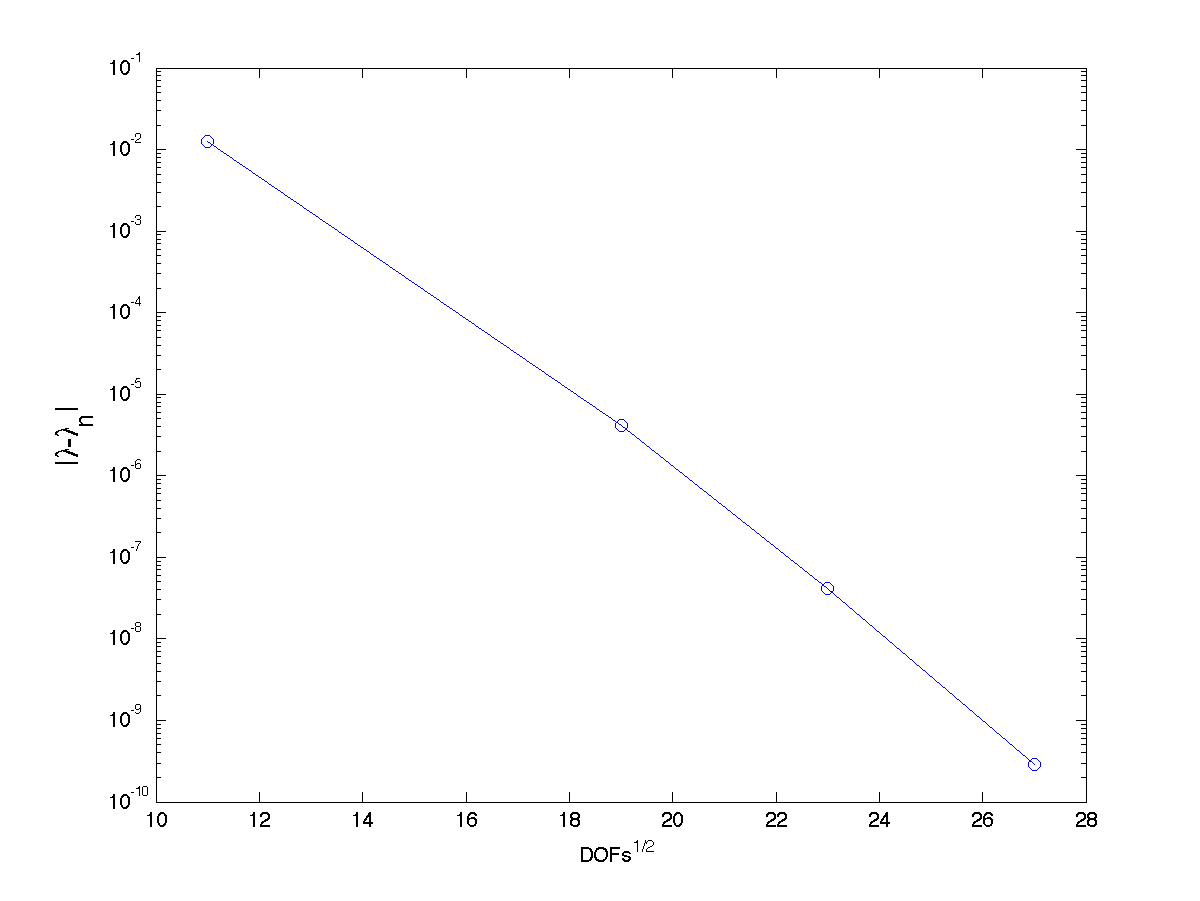
\includegraphics[width=0.8\textwidth]{img/ex_2.png}
\end{center}
\vspace{-5mm}
\caption{Convergence plot for the fifth eigenvalue.}
\label{fig:conv_eig5}
\end{figure}

%\begin{figure}[!ht]
%\begin{center}
%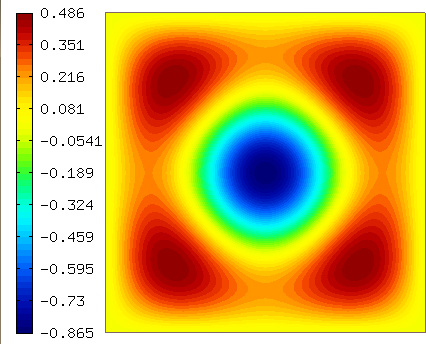
\includegraphics[width=0.8\textwidth]{img/ex_2_paper.png}
%\end{center}
%\vspace{-5mm}
%\caption{Eigenfunction of the fifth eigenvalue.}
%\label{fig:sol_eig5}
%\end{figure}

However, when the standard orthogonality is used, five eigenpairs are computed on each adapted mesh, this means that overall 20 eigenpairs are computed. This is quite expensive, but the cost can be reduced using the improved orthogonality, see Section~\ref{sec:imp_ortho}. The convergence rate is exactly the same as in Figure~\ref{fig:conv_eig5}, but the number of computed eigenpairs is dramatically smaller. In Table~\ref{tab:imp_orhto} we reported the number of computed eigenpairs on each adapted mesh using either the standard or the improved orthogonality.
It is worth to say that if we had used the eigensolver on the meshes, we would have computed five eigenpairs for each mesh, as the standard orthogonality.

\begin{table}[h]
\begin{center}

\begin{tabular}{|c|c|c|}
\hline
$n$ &  Standard &Improved\\
\hline
\hline
1 & 5 & 2\\
\hline
2 & 5 & 2\\
\hline
3 & 5 & 2\\
\hline
4 & 5 & 2\\
\hline \hline
\bf{Total} & 20 & 8\\
\hline
\end{tabular}
\end{center}

\caption{Number of computed eigenpairs for different orthogonality technologies.}\label{tab:imp_orhto}
\end{table}


\section{Reproducibility of Results} \label{sec:reproducibility}

The method presented in this paper is part of the open source C++ library 
Hermes (http://hpfem.org/hermes), and it can be found in 
example "eigen-adapt-iter". Whoever
has a problem with building the library on his/her computer, or with running 
this example, should send
a message to the mailing list hermes2d@googlegroups.com. For a model 
implementation of the Anderson acceleration technique mentioned in Section 
\ref{sec:picard++} visit the FEMhub Online Lab (http://femhub.org), where
it is part of the Published Worksheet "Fixed Point Iteration (with Acceleration)".
In the Online Lab, anyone can freely experiment with the technique. The 
Online Lab is powered with a 60-processor computer at the University of 
Nevada, Reno.

\section{Conclusion and Outlook}\label{sec:conclusion}

We presented a novel adaptive higher-order finite element method ($hp$-FEM) 
for PDE eigenproblems. As opposed to conventional methods, it does not need
to call an eigensolver in each adaptivity step. This eliminates standard 
problems associated with repeated eigenvalues. The technique also makes it 
possible to approximate different eigenfunctions on individual meshes. 
The fact that one mesh cannot be optimal for multiple eigenfunctions at the
same time was the original motivation for this study. Another motivation is 
that using the present method, many eigenfunctions can be calculated separately 
in parallel, without a parallel eigensolver. In our next steps we will continue 
along this line and adjust the adaptive multimesh $hp$-FEM technique \cite{solin2} 
to approximate multiple eigenfunctions adaptively on individual meshes.

\section*{Acknowledgment}

The first author was supported by the Subcontract No. 00089911 of Battelle Energy
Alliance (U.S. Department of Energy intermediary) as well as by the Grant No. 
IAA100760702 of the Grant Agency of the Academy of Sciences of the Czech Republic.


\clearpage

\begin{thebibliography}{[KLR73]}

\bibitem{anderson}
D. G. Anderson. Iterative procedures for nonlinear integral equations. J. Assoc. Comput.
Machinery, 12:547–560, 1965.

\bibitem{dubcova1}
L. Dubcova, P. Solin, G. Hansen, H. Park: Comparison of Multimesh $hp$-FEM 
to Interpolation and Projection Methods for Spatial Coupling of Reactor 
Thermal and Neutron Diffusion Calculations, J. Comput. Phys. 230 (2011) 1182-1197.

\bibitem{giani1}
S. Giani, I.G. Graham: A convergent adaptive method for elliptic eigenvalue 
problems. SIAM J. Numer. Anal. 47 (2009), 1067-1091.

\bibitem{solin1} 
P. Solin, D. Andrs, J. Cerveny, M. Simko: 
PDE-Independent Adaptive $hp$-FEM Based on Hierarchic Extension of Finite Element Spaces.
J. Comput. Appl. Math. 233 (2010) 3086-3094.

\bibitem{solin2} 
P. Solin, J. Cerveny, L. Dubcova, D. Andrs: Monolithic Discretization of Linear 
Thermoelasticity Problems via Adaptive Multimesh $hp$-FEM, J. Comput. Appl. Math 
234 (2010) 2350-2357.

\bibitem{solin3}
P. Solin, K. Segeth, I. Dolezel: {\em Higher-Order Finite Element Methods},
Chapman \& Hall / CRC Press, 2003.

\bibitem{BaOs:87}
I.~Babu\v{s}ka and J.~Osborn.
\newblock {\em Estimates for the errors in eigenvalue and eigenvector
  approximation by Galerkin methods, with particular attention to the
  case of multiple eigenvalues}, 
\newblock{\em SIAM J. Numer. Anal.}, 24:1249-1276, 1987.

\bibitem{BaOs:89}
I.~Babu\v{s}ka and J.~Osborn.
\newblock {Finite element-Galerkin approximation of the
  eigenvalues and eigenvectors of selfadjoint problems}, 
\newblock{\em Math. Comput.} 186:275-297, 1989.
 
\bibitem{strang}
G.~Strang and G.~J. Fix.
\newblock {\em An Analysis of the Finite Element Method}.
\newblock Prentice-Hall, 1973.

\bibitem{babuska}
I.~Babu\v{s}ka and J.~Osborn.
\newblock {\em Eigenvalue Problems}.
\newblock in Handbook of Numerical Analysis Vol II, eds P.G. Cairlet and J.L. Lions, North Holland, 1991.

\bibitem{hackbusch}
W.~Hackbusch.
\newblock {\em Elliptic Differential Equations}.
\newblock Springer, 1992.

\bibitem{conv_sinum}
S. Giani and Ivan G. Graham,
\newblock {A Convergent Adaptive Method for Elliptic Eigenvalue Problems},
\newblock{\em SIAM J. Numer. Anal.} 47(2):1067-1091, 2009.

\bibitem{schwab}
C. Schwab,
\newblock {$p$- and $hp$- finite element methods},
\newblock{\em Oxford University Press}, 1998.

\bibitem{arpack}
R. B. Lehoucq, D. C. Sorensen, and C. Yang, \newblock{ARPACK
Users' Guide: Solution of Large-Scale Eigenvalue Problems with
Implicitly Restarted Arnoldi Methods}, \newblock {(SIAM, 1998)}.

\bibitem{newton}
H.~R\"{o}ck,
\newblock{Finfding an eigenvector and eigenvalue, with Newtons method for solving systems of nonlinear equations},
\newblock{\em  Report CMDIE WS2002/03}

\bibitem{pcf_apost}
S.~Giani and I.~G.~Graham,
\newblock {Adaptive finite element methods for computing band
gaps in photonic crystals},
\newblock{\em Numerische Mathematik}, submitted.


\bibitem{lalor_prediction_2007}
N.~Lalor and H-H.~Priebsch
	\newblock {The prediction of low- and mid-frequency internal road vehicle noise: a literature survey},
	\newblock{\em Proceedings of the Institution of Mechanical Engineers, Part D: Journal of Automobile Engineering} 221(3):245--269, 2007.

\bibitem{berini_plasmon-polariton_2000}
P.~ Berini
	\newblock{Plasmon-polariton waves guided by thin lossy metal films of finite width: Bound modes of symmetric structures},
	\newblock{\em Physical Review B} 61(15):10484+, 2000.

\bibitem{JoMeWi:95} 
J. D. Joannopoulos, R. D. Meade, and J. N. Winn, 
\newblock{Photonic Crystals. Molding the Flow of Light} 
\newblock{Princeton
Univ. Press, Princeton, NJ}, 1995.

\bibitem{cliffe_adaptive_2010}
A.~Cliffe, E.~Hall and P.~Houston
	\newblock{Adaptive Discontinuous Galerkin Methods for Eigenvalue Problems Arising in Incompressible Fluid Flows},
	\newblock{\em {SIAM} Journal on Scientific Computing} 31(6):4607--4632, 2010.

\end{thebibliography}



\end{document}

%%
%% End of file `elsarticle-template-num.tex'.
